% ===================================================================================================
%                                                 |                                                 |
%                                                 |                                                 |
% -------------------------------------------- SECTION ---------------------------------------------|
%                                                 |                                                 |
%                                                 |                                                 |
% ===================================================================================================
\section{Mathematical framework}\label{sec:transfer_learning}
The goal in this section is to model the scaling in the energy and time demand that results from the use of several robots performing numerous skills.

% ===================================================================================================
\subsection{Energy and time demand for learning skills}
% ---
\begin{figure}[!ht]
	\centering
	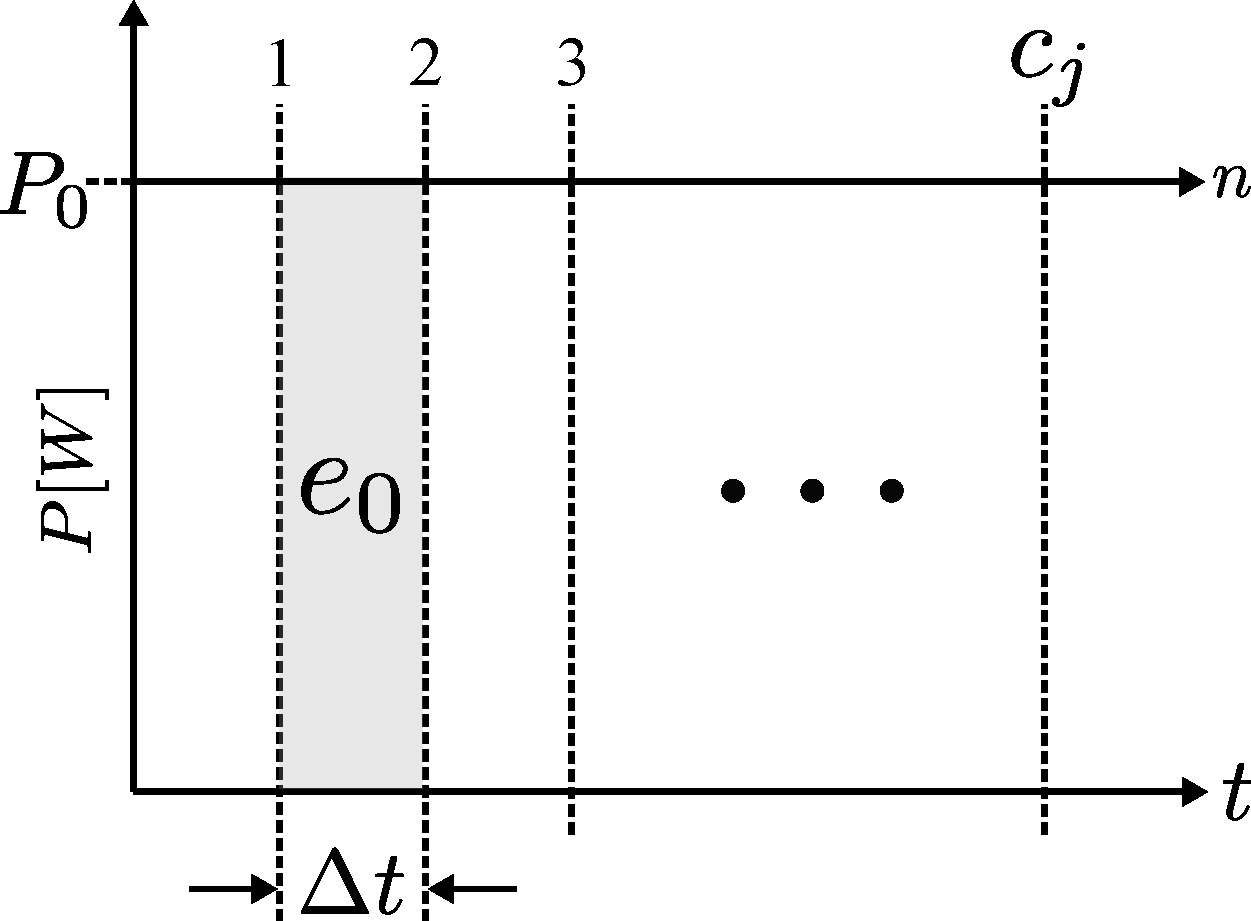
\includegraphics[width=0.9\columnwidth]{fig/power_per_episode.pdf}
	\caption{Power consumption per episode.}
	\label{fig:power_per_episode}
\end{figure}
%---
\begin{tcolorbox}
\begin{definition}\label{definition:complexity} The complexity $c_j$ of a skill $ s_j $  is understood as the number of trial episodes $n$ needed to successfully learn the skill; i.e., all actions and states visited until a stopping criterion is reached. 
\end{definition}
\end{tcolorbox}
% ---
Now, let $P_0$ be the total power\footnote{$P_0$ is assumed to be constant.} required by the robot to sustain the learning process. Furthermore,
% ---
\begin{tcolorbox}
\begin{assumption}\label{assumption:time} Every trial episode $n$ takes the same amount of time $\Delta t$ to be executed (Fig.~\ref{fig:power_per_episode}).
\end{assumption}
\end{tcolorbox}
% ---
% ---------------------------------------------------------------------------------------------------
\subsubsection{\textbf{Energy requirement}}
Under Assumption \ref{assumption:time}, the energy consumption of the $n$-th episode $e^{(n)}_j$ is simply
% ---
\begin{equation}\label{eq:energy_per_episode}
    e^{(n)}_j = \cancelto{\text{const}}{P_0\cdot \Delta t} = e_0.
\end{equation}
% ---
Consequently, the energy consumed by a robot learning the skill $ s_j $ is directly proportional to the complexity; i.e.
% ---
\begin{equation}\label{eq:energy_per_skill}
    E_j =\sum_{n=1}^{c_j} e^{(n)}_j = e_0 \cdot c_j.
\end{equation}
% ---
Having $\mathcal{S}$ represent the set of all \emph{to-be-learned} skills, with $|\mathcal{S}| = N_\mathcal{S}$; then, the energy spent on learning $\mathcal{S}$ is
% ---
\begin{equation}\label{eq:total_energy}
	E_{\mathcal{S}} = \sum_{j=1}^{{N_{\mathcal{S}}}} E_j = e_0 \sum_{j=1}^{{N_{\mathcal{S}}}} c_j%N_{\mathcal{T}} \cdot e_0 \cdot c_j 
\end{equation}
% ---
% ---------------------------------------------------------------------------------------------------
\subsubsection{\textbf{Time requirement}}
Similarly, the total time $T_{\mathcal{S}}$ is simply
% ---
\begin{equation}\label{eq:total_energy}
	T_{\mathcal{S}} = \Delta t \sum_{j=1}^{{N_{\mathcal{S}}}} c_j.
\end{equation}
% ---
% ===================================================================================================
\subsection{Similarity and knowledge}
%---
\begin{tcolorbox}
	\begin{assumption}\label{assumption:skill_clustering} When the degree of similarity among a set of skills is comparable, they can be clustered together.
		\end{assumption}
\end{tcolorbox}
% ---
Following Asm.~\ref{assumption:skill_clustering}, let $\mathcal{S}_k \subset \mathcal{S}$ be a subset of skills that share high similarity; i.e. a \emph{cluster} of skills. Furthermore, consider another set $\mathcal{Z}_k \subset \mathcal{S}_k$ that denotes already learned skills from $\mathcal{S}_k$. Asm.~\ref{assumption:skill_clustering} implies that a new skill $s_{j,k} \in \mathcal{S}_k$ can always benefit from the knowledge contained in $\mathcal{Z}_k$. This implies that the more skills enter $\mathcal{Z}_k$ (with $|\mathcal{Z}_k| = N_{j,k}$), the less knowledge about $ s_{j,k} $ will remain to be learned.

Now, we introduce a function \hl{$\bar{\sigma}_{j,k}(\mathcal{Z}_k)\in [0,1]$ that expresses the knowledge about a skill $s_{j,k} \in \mathcal{S}_k$ that \textbf{is not} contained in $\mathcal{Z}_k$; i.e. $s_{j,k} \notin \mathcal{Z}_k$}. The function $\bar{\sigma}_{j,k}(\cdot)$ satisfies:
\begin{itemize}
	\item $\bar{\sigma}_{j,k}(\mathcal{Z}_k) = 1$, if $\mathcal{Z}_k=\emptyset$ or if it does not contain knowledge about the skill $s_{j,k}$
	\item $\bar{\sigma}_{j,k}(\mathcal{Z}_k) = 0$, if \emph{all} the knowledge about skill $s_{j,k}$ is contained in $\mathcal{Z}_k$
\end{itemize} 
Conceptually, $\bar{\sigma}_ {j,k}(\mathcal{Z}_k)$ is the fraction of knowledge that remains to be learned \hl{about the $k$-th cluster}.
% ---------------------------------------------------------------------------------------------------
\subsubsection{\textbf{Leveraging the acquired knowledge}}
To simplify the analysis, we introduce a fundamental complexity
\begin{tcolorbox}
\begin{assumption}\label{assumption:fundamental_complexity} The fundamental complexity $c_0$ describes the maximum number of episodes required to learn \emph{any} skill.
\end{assumption}
\end{tcolorbox}
% ---
If, in learning a skill $ s_{j,k} $, a robot uses the knowledge contained in $\mathcal{Z}_k$ about $s_{j,k}$; then, its associated complexity $ c_j $ is a scaled-down version of the complexity $c_{0}$ and is given by:
% ---
\begin{equation}\label{eq:scaled_complexity}
c_{j,k} = c_{0} \cdot \bar{\sigma}_{j,k}\left(\mathcal{Z}_k\right)\in [0, c_{0}].
\end{equation}
%---
% \begin{tcolorbox}
% 	\begin{assumption}\label{assumption:skill_complexity}
% 		The skills in $ \mathcal{S} $ share a high degree of similarity (have the same complexity).
% 	\end{assumption}
% \end{tcolorbox}
% ---
% Assumption~\ref{assumption:skill_complexity} implies that a new skill $s_j \in \mathcal{S}$ can always benefit from the knowledge contained in $\mathcal{Z} \subset \mathcal{S}$. This implies that the more skills enter $\mathcal{Z}$ (with $|\mathcal{Z}| = N_j$), the less knowledge about $ s_j $ will remain to be learned.

According to \eqref{eq:scaled_complexity} the complexity scales down as a function of the number of learned skills, as exemplified in Fig.~\ref{fig:complexity_per_cardinality}. Alternatively,
% ---
\begin{equation}\label{eq:knowledge_limit}
    \lim_{N_{j,k}\to N_{\mathcal{S}_k}} \bar{\sigma}_ {j,k} = 0 \implies \lim_{N_{j,k}\to N_{\mathcal{S}_k}} c_{j,k} = 0.
\end{equation}

%Furthermore, consider the following assumptions
%% ---
%\begin{tcolorbox}
%	\begin{assumption}\label{assumption:skill_clustering} When the degree of similarity among a set of skills is comparable, they can be clustered together.
%	\end{assumption}
%\end{tcolorbox}
%% --- 
%The previous assumption is depicted in Fig.~\ref{fig:incremental_transfer_similarity} where similar skills are grouped together in four different clusters.
\begin{tcolorbox}
	\begin{assumption}\label{assumption:exponential_decrease} The knowledge function $\bar{\sigma}(\cdot)_{j,k}$ has a monotonically decreasing behavior.
	\end{assumption}
\end{tcolorbox} 
% ---
Considering Asm.~\ref{assumption:exponential_decrease}, an idealization of the behavior described by \eqref{eq:knowledge_limit} can be modeled as a decreasing exponential, which is a function of the number of already learned skills $N_{j,k}$:% from the cluster $k$; i.e. ${^kN_j}$:
% ---
\begin{equation}\label{eq:incremental_knowledge}
     \boxed{\bar{\sigma}_{j,k} = \left(e^{-\alpha |\mathcal{Z}_k|}\right)^r = \left(e^{-\alpha  \cdot N_{j,k}}\right)^r \in (0,1],}
\end{equation}
% ---
where $ 0<\alpha<<1$ models how effectively the knowledge contained in $\mathcal{Z}_k$ is shared with $s_{j,k}$ and $r$ represents the number of agents \emph{concurrently} gathering and sharing knowledge.

% ===================================================================================================
\subsection{Knowledge sharing under different learning paradigms}
The following assumptions are analogous to average behavior and imply that a suitable scaling strategy is available and executed.
% ---
\begin{tcolorbox}
	\begin{assumption}\label{assumption:agent_similarity}
		Every agent has the same abilities and energetic cost.
	\end{assumption}
\end{tcolorbox}
% %---
% \begin{tcolorbox}
% 	\begin{assumption}\label{assumption:skill_clustering} When the degree of similarity among a set of skills is comparable, they can be clustered together.
% 		\end{assumption}
% \end{tcolorbox}
% % ---
\begin{tcolorbox}
	\begin{assumption}\label{assumption:cluster_size}
		Every cluster contains the same number of skills.
	\end{assumption}
\end{tcolorbox}
% ---
\begin{tcolorbox}
	\begin{assumption}\label{assumption:cluster_transferability}
		The knowledge transferability between skills is assumed to be equal; therefore, also the transferability between clusters is assumed to be equal.
	\end{assumption}
\end{tcolorbox}
% ---------------------------------------------------------------------------------------------------
\subsubsection{\textbf{Isolated learning (Iso)}} a robot learns all the skills in $\mathcal{S}$ one after another from scratch, disregarding the knowledge from all other learned skills in $\mathcal{Z}_k$ when learning a new skill. In other words, this implies that $N_{j,k} = 0$ in \eqref{eq:incremental_knowledge}. Therefore, the energy required by the robot to learn all skills in $\mathcal{S}$ is simply
% ---
% \begin{align}
%     \begin{split}
%       E^{(Iso)}_{\mathcal{S}} &= N_{\mathcal{S}} \cdot E^{(Iso)}_j\\ 
%       &= N_{\mathcal{S}} \cdot e_{0} \cdot \cancelto{c_{0}}{c_{j}} 
%     \end{split}
% \end{align}
\begin{align}
    \begin{split}
      E^{(Iso)}_{\mathcal{S}} &= N_{\mathcal{S}} \cdot E^{(Iso)}_j = N_{\mathcal{S}} \left(  e_{0} \cdot c_0 \right)
    \end{split}
\end{align}
% ---
Furthermore, using batches of $m$ robots to learn $m$ skills in parallel, needs 
% ---
\begin{equation}
    ^{\lvert \lvert}E^{(Iso)}_\mathcal{S}= \underbrace{m}_{\text{robots}}\cdot \overbrace{\frac{E^{(Iso)}_\mathcal{S}}{m}}^{\text{energy per robot}} = E^{(Iso)}_\mathcal{S}
\end{equation}
% ---
Therefore, there are no energy reductions under this scheme.

%---
% \begin{figure}[!ht]
% 	\centering
% 	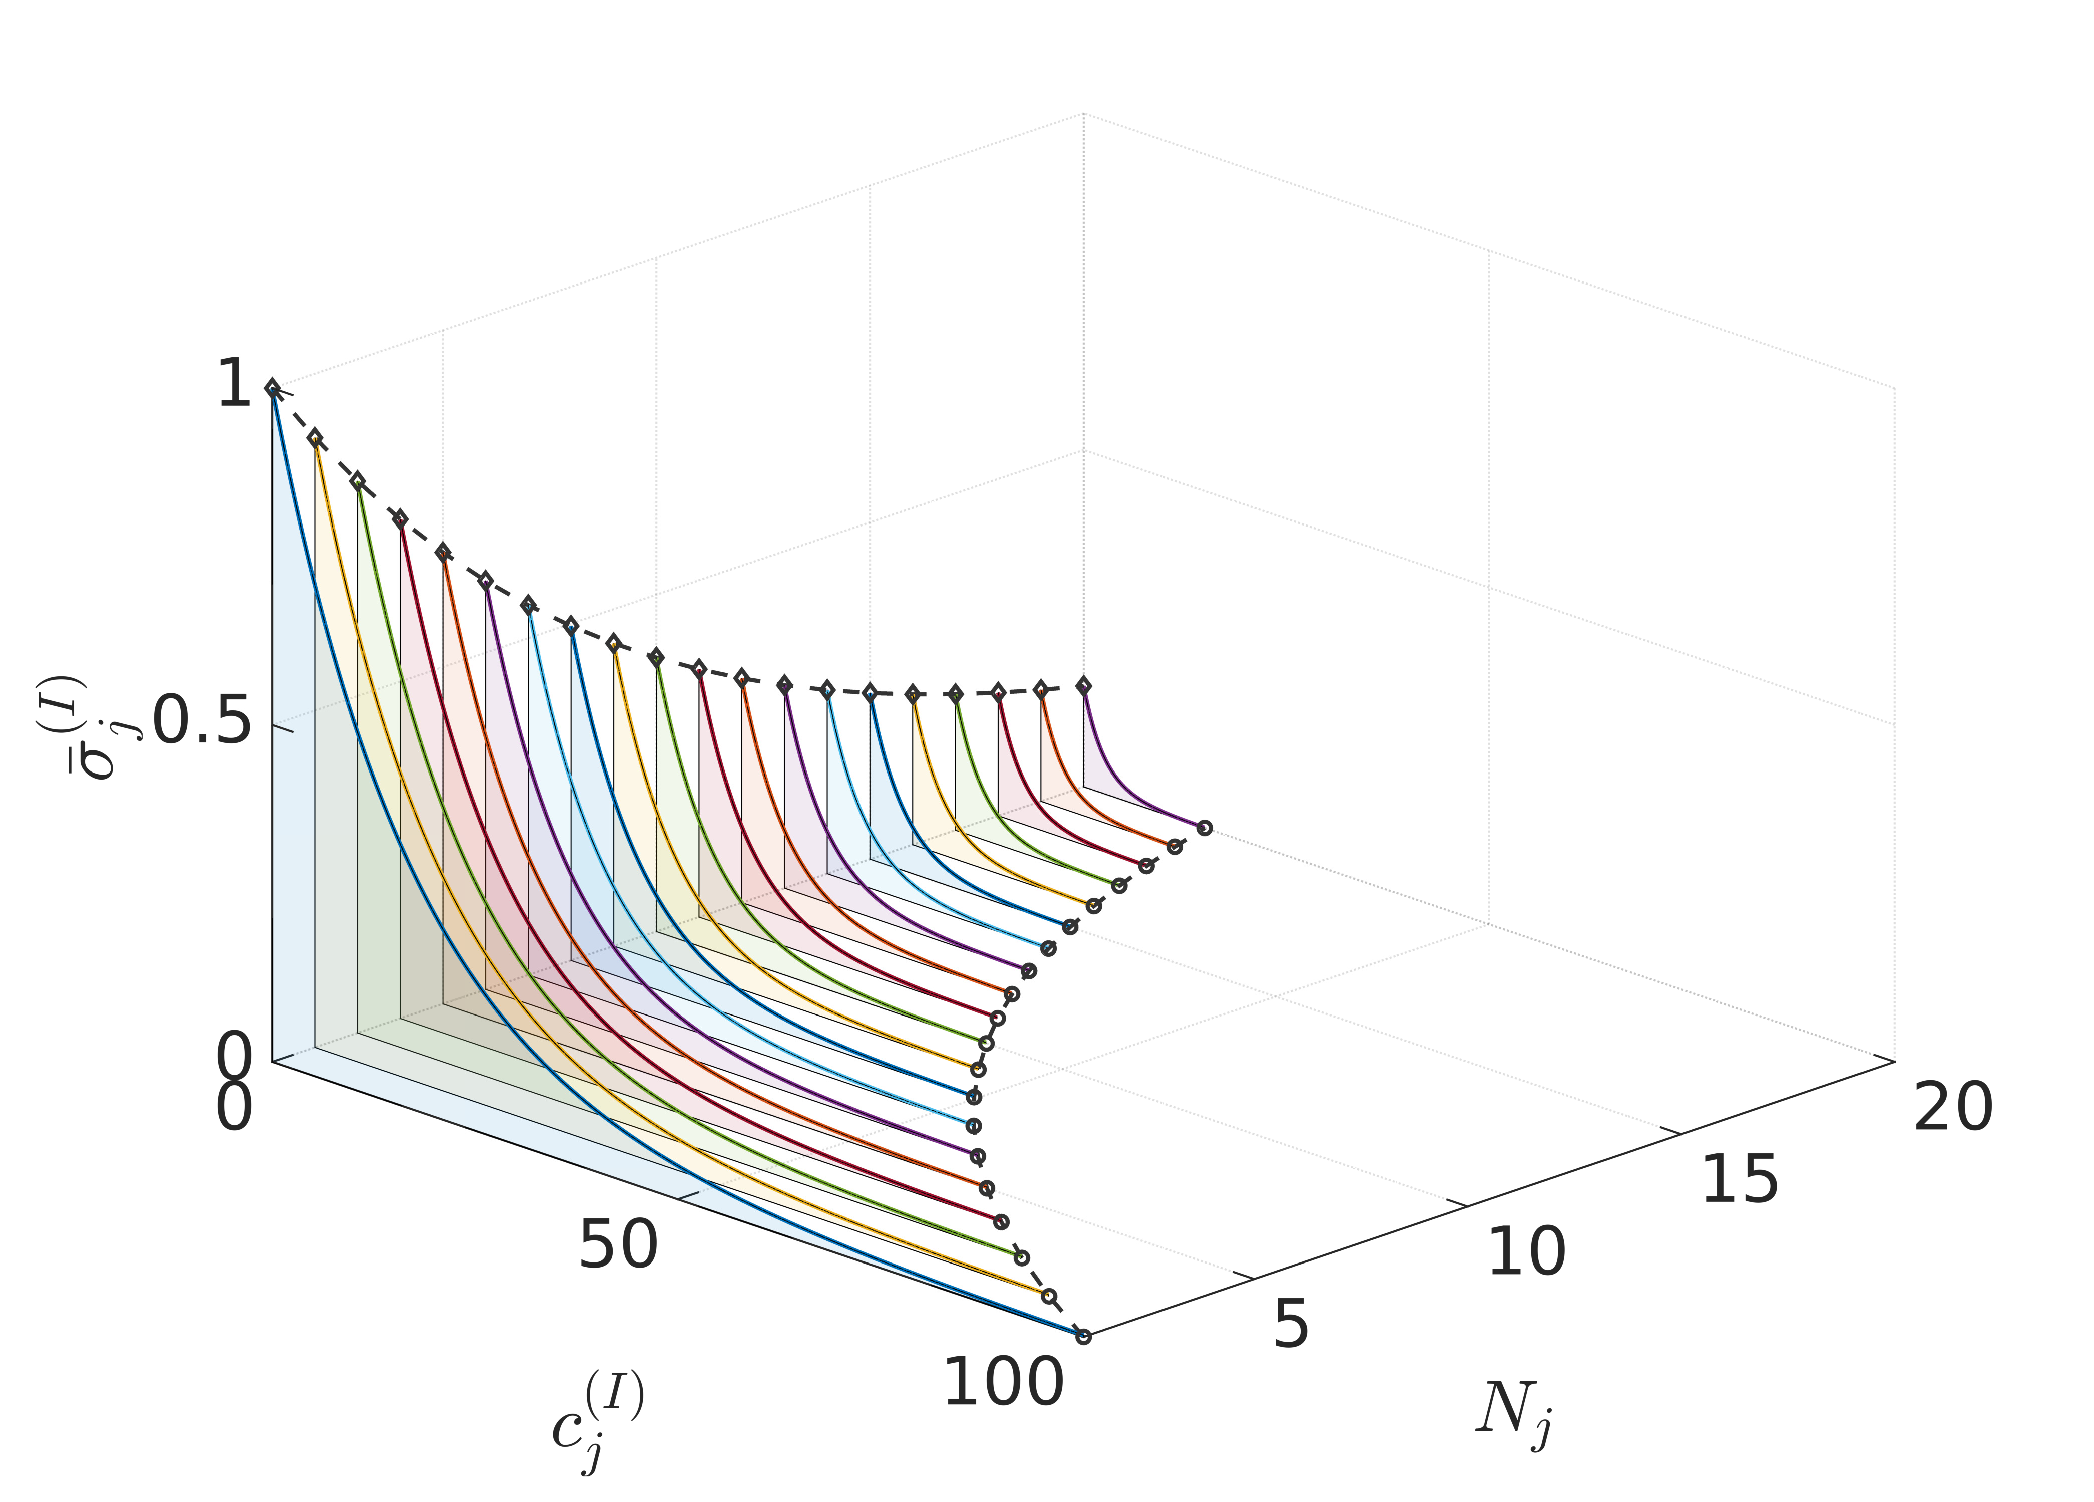
\includegraphics[width=0.99\columnwidth]{tex/fig/single_incremental_knowledge.pdf}
% 	\caption{Knowledge sharing in incremental learning. A single agent leverages previously acquired knowledge from other learned skills in $\mathcal{Z}$.}
% 	\label{fig:single_incremental_knowledge}
% \end{figure}
%---
\begin{figure}[!ht]
	\centering
	\includegraphics[width=0.8\columnwidth]{tex/fig/complexity_incremental.pdf}
	\caption{In IL the complexity of a skill $c^{(I)}_{j,k}$ (number of trial episodes) decreases exponentially with the number of learned skills $|\mathcal{Z}_k|=N_{j,k}$.}
	\label{fig:complexity_per_cardinality}
\end{figure}
% ---
% ---
\begin{figure}[!t]
	\centering
	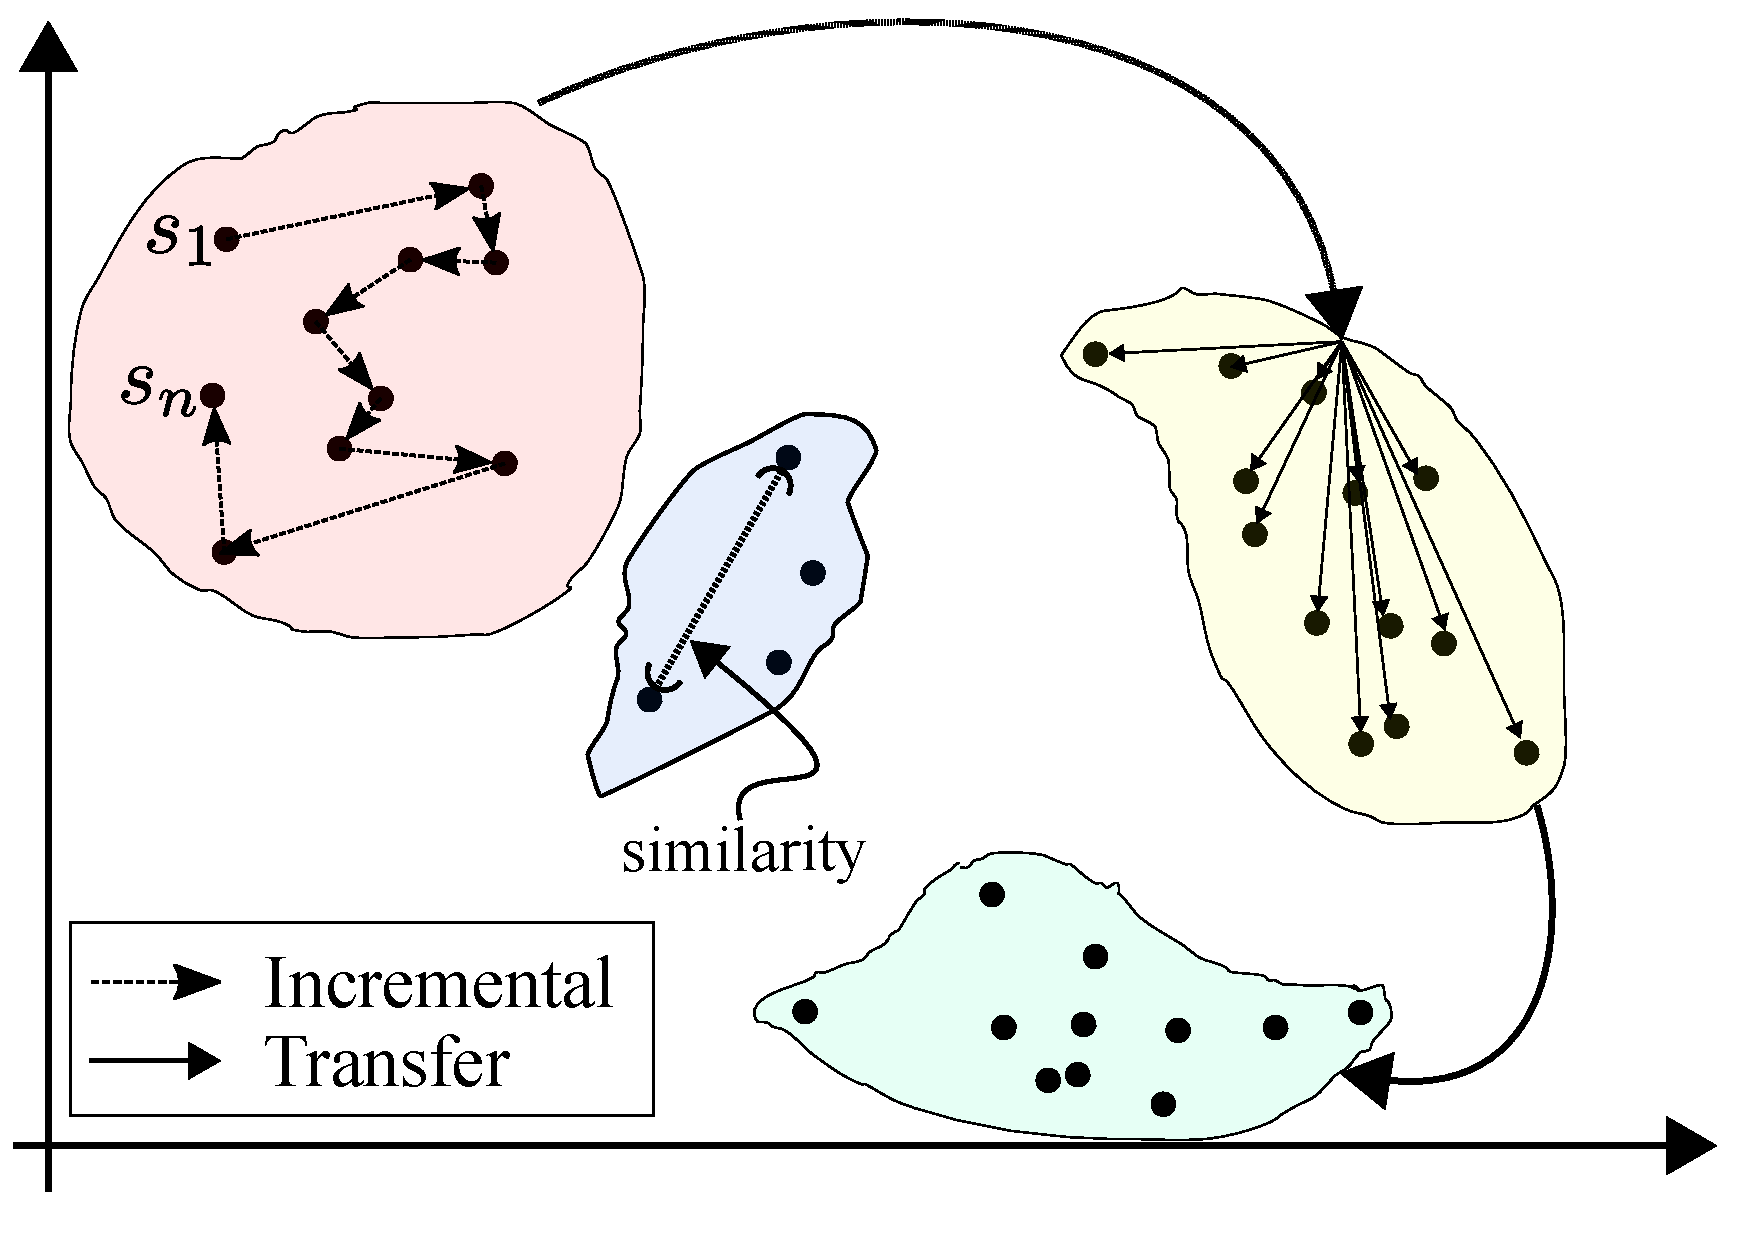
\includegraphics[width=0.9\columnwidth]{fig/incremental_transfer_similarity_v2.pdf}
	\caption{Incremental and transfer learning and its relation to similarity.}
	\label{fig:incremental_transfer_similarity}
\end{figure}
% ---
% ---
\begin{figure*}[!htb]
	\centering
	\hspace*{\fill}
	\subfloat[]{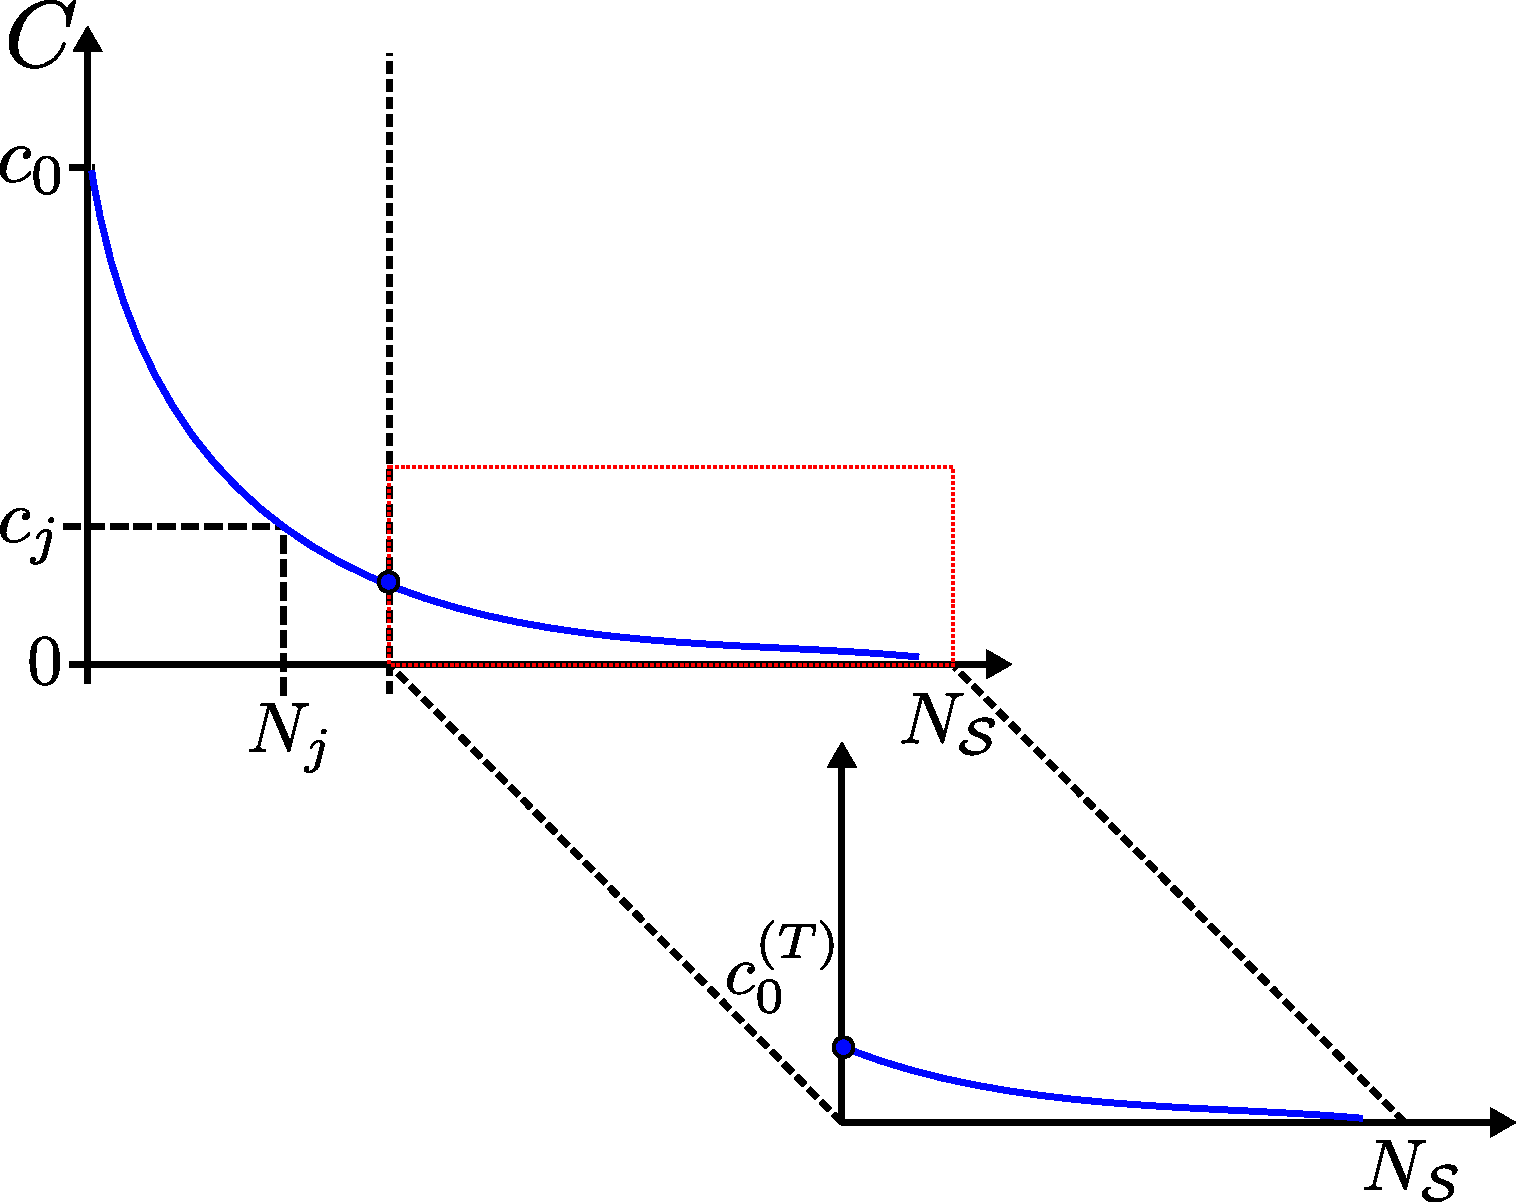
\includegraphics[width= 0.80\columnwidth]{fig/effect_transfer_learning.pdf} \label{fig:effect_transfer_learning}}  
	\hfill
	\subfloat[]{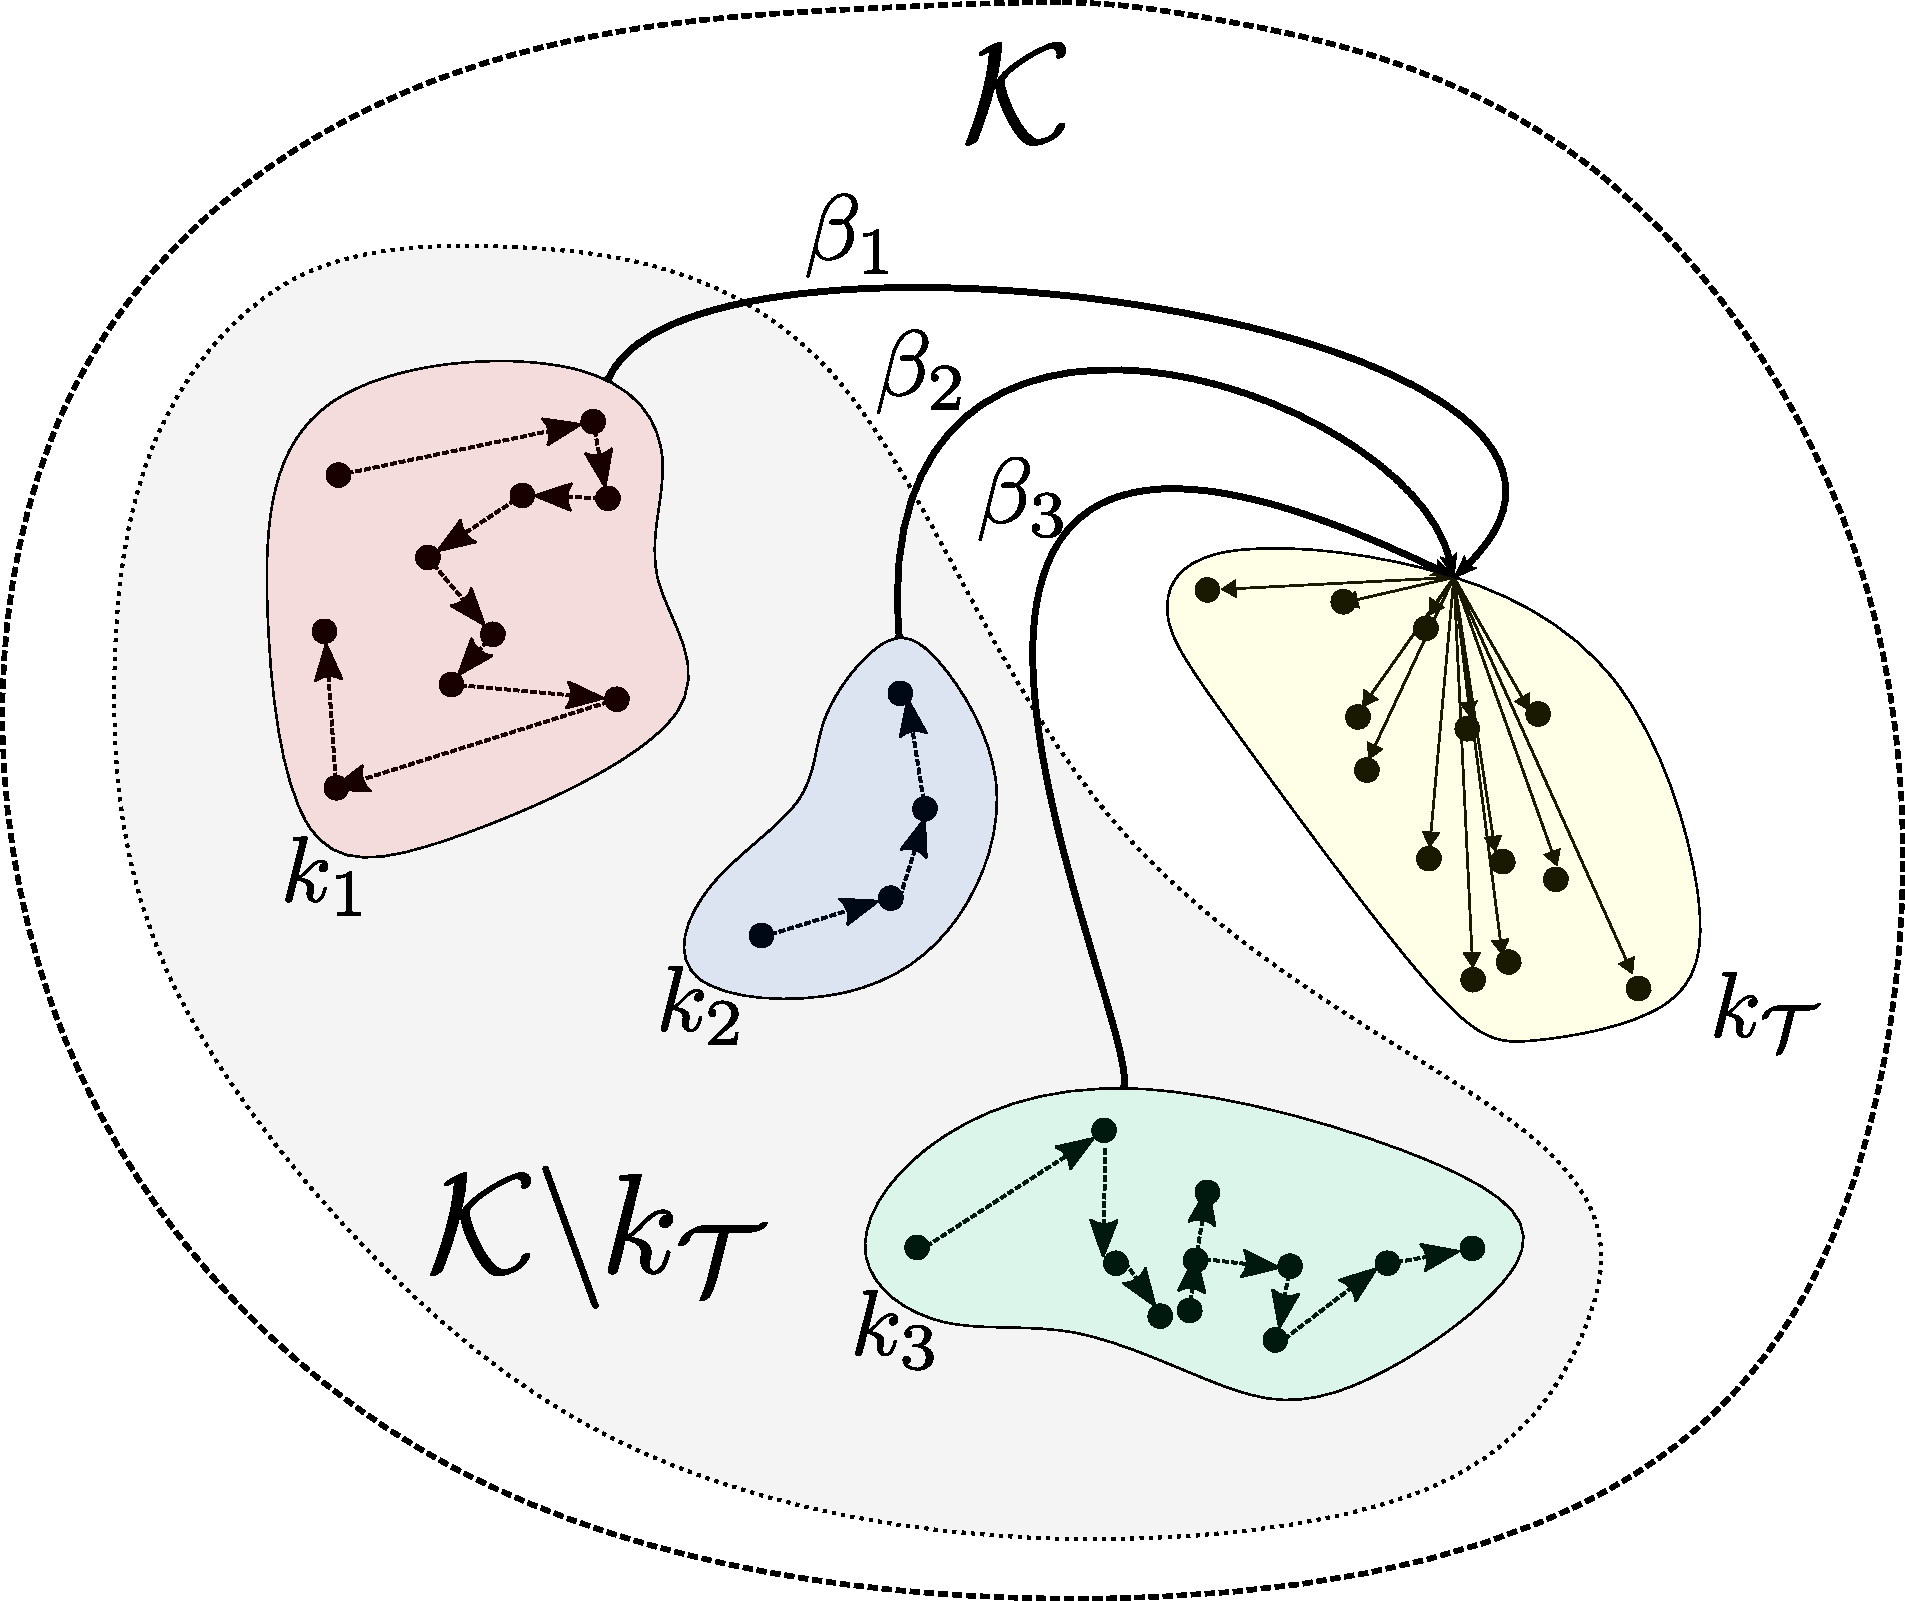
\includegraphics[width= 0.80\columnwidth]{tex/fig/cluster_knowledge_transfer_v3.pdf} \label{fig:cluster_knowledge_transfer}}
	\hspace*{\fill}
	\caption[] {\label{fig:tranfer_learninhg} Transfer learning. \subref{fig:effect_transfer_learning} The effect of transfer learning, \subref{fig:cluster_knowledge_transfer} transfer of knowledge from different origin clusters to the target cluster.}
\end{figure*}
% ---
% ---------------------------------------------------------------------------------------------------
\subsubsection{\textbf{Incremental learning (I)}}
referring back to Asm.~\ref{assumption:skill_clustering}, skills with comparable similarity are clustered in $\mathcal{K} = \lbrace k_i \rbrace^{N_\mathcal{K}}_{i=1} $ clusters, with $N_\mathcal{K}$ being the total number of clusters, see Fig.~\ref{fig:incremental_transfer_similarity}. Any two skills belonging to different clusters profit negligibly from incremental learning algorithms in virtue of their relatively low similarity. \textcolor{red}{Furthermore, as the agent has access only to its previously collected knowledge, $r = 1$ in \eqref{eq:incremental_knowledge}}. Therefore, the scaling effect that incremental learning has on the skill complexity $c_{j,k}$ for the skills contained in the $k$-th cluster is

% ---
% \begin{equation}\label{eq:complexity_IL}
%  {^k}c^{(I)}_j = c_0 \cdot {^k}\bar{\sigma}_j = c_0 \left( e^{-\alpha \cdot {^kN_{j}}}\right)^r = c_0 \left( e^{-\alpha \cdot {^kN_{j}}}\right),
% \end{equation}
% \begin{equation}\label{eq:complexity_IL}
% 	c^{(I)}_{j,k} = c_0 \cdot \bar{\sigma}_{j,k} = c_0 \left( e^{-\alpha \cdot {N_{j,k}}}\right)^r = c_0 \left( e^{-\alpha \cdot {N_{j,k}}}\right),
% \end{equation}
\begin{equation}\label{eq:complexity_IL}
	c^{(I)}_{j,k} = c_0  e^{-\alpha \cdot {N_{j,k}}}.
\end{equation}
% ---
%\textcolor{red}{where $r=1$} and 
% ${N_{j,k}}$ indicates the number of already learned skills in the $k$-th cluster. 
This effect is shown in Fig.~\ref{fig:complexity_per_cardinality}, which obeys Asm.~\ref{assumption:fundamental_complexity} and \ref{assumption:exponential_decrease}. %Similarly, $\bar{\sigma}_{j,k}$ indicates the knowledge that is yet to be acquired about a given skill in cluster $k$. \textcolor{red}{In virtue of the high similarity of the skills in the cluster, the term $\left(1-\bar{\sigma}_{j,k}\right)$ indirectly reflects the knowledge collected from the skills in the $k$-th cluster.}

The total number of trial episodes $ C_k $ that an agent following an incremental learning strategy needs to learn the skills in a cluster $ k $ is given by
% ---
%\begin{align}
%	\begin{split}
%		C^{(I)}_k &= \sum^{N_\mathcal{S}/N_\mathcal{K}}_{j=1} c_0 \cdot e^{-\alpha \cdot {^kN_{j}}} = \sum^{N_\mathcal{S}/N_\mathcal{K}}_{j=1}c_0 \cdot e^{-\alpha {^{k}\cancelto{j-1}{N_{j}}}}\\
%		&= c_0 \sum^{N_\mathcal{S}/N_\mathcal{K}}_{j=1} e^{-\alpha (j-1)}.
%	\end{split}
%\end{align}
\begin{align}
	\begin{split}
		C^{(I)}_k &= \sum^{N_\mathcal{S}/N_\mathcal{K}}_{j=1} c^{(I)}_{j,k}  \\
		&= \sum^{N_\mathcal{S}/N_\mathcal{K}}_{j=1} c_0 \cdot  \bar{\sigma}_{j,k}  = \sum^{N_\mathcal{S}/N_\mathcal{K}}_{j=1} c_0 e^{-\alpha {\cancelto{j-1}{N_{j,k}}}}\\
		&= c_0 \sum^{N_\mathcal{S}/N_\mathcal{K}}_{j=1} e^{-\alpha (j-1)}=c_0 \frac{1 - e^{-\alpha \frac{N_\mathcal{S}}{N_\mathcal{K}}}}{1 - e^{-\alpha}},
	\end{split}
\end{align}
% ---
where $N_{\mathcal{S}_k} = N_\mathcal{S}/N_\mathcal{K}$ as per Asm.~\ref{assumption:cluster_size}\footnote{The equality $N_{j.k} = j-1$ is based on a previous ordering of the skills in $\mathcal{S}_k$.}. Likewise, the total number of episodes to learn the skills in all the $ N_\mathcal{K} $ clusters is
%\begin{align}\label{eq:complexity_incremental_single}
%	\begin{split}
%	C^{(I)} &= N_\mathcal{K} \cdot c_0 \frac{1 - e^{-\alpha \frac{N_\mathcal{S}}{N_\mathcal{K}}}}{1 - e^{-\alpha}}\\
%&= N_\mathcal{K} \cdot c_0 \frac{1 - \bar{\sigma}^{(I)}}{1 - e^{-\alpha}}.
%	\end{split}
%
%\end{align}
\begin{align}\label{eq:complexity_incremental_single}
	\begin{split}
		C_\mathcal{S}^{(I)} &= N_\mathcal{K} \cdot c_0 \frac{1 - e^{-\alpha \frac{N_\mathcal{S}}{N_\mathcal{K}}}}{1 - e^{-\alpha}}\\ 
		&= N_\mathcal{K} \cdot c_0 \frac{1 - \bar{\sigma}_k^{(I)}}{1 - e^{-\alpha}}.
	\end{split}
\end{align}
% ---
with $ \overbrace{\bar{\sigma}^{(I)}_k = e^{-\alpha \frac{N_\mathcal{S}}{N_\mathcal{K}}}}^{\text{isn't this supposed to be 0?}} $ representing the knowledge remaining after learning all the skills in a cluster. If $ m $ robots are available, each agent can take care of learning $ \frac{N_\mathcal{S}}{m \cdot N_\mathcal{K}} $ skills in parallel with the rest. Under such conditions, the total number of episodes is simply
% ---
\begin{align}\label{eq:complexity_incremental_parallel}
	\begin{split}
		{}^{\lvert \lvert}C_\mathcal{S}^{(I)} &= m \left( N_\mathcal{K} \cdot c_0 \frac{1 - e^{-\alpha \frac{N_\mathcal{S}}{m \cdot N_\mathcal{K}}}}{1 - e^{-\alpha}}\right) \\&= m \left( N_\mathcal{K} \cdot c_0 \frac{1 - \left(\bar{\sigma}^{(I)}_k\right)^{\frac{1}{m}} }{1 - e^{-\alpha}} \right) \\
		&= m \cdot N_\mathcal{K} \cdot c_0 \frac{1 - \bar{\sigma}^{(I)}_m}{1 - e^{-\alpha}} 	
	\end{split}	
\end{align}
%---
\begin{table*}[htbp!]
	\begin{center}
		\captionof{table}{The total complexity of the different learning schemes.} \label{tab:method_comparison}
		\begin{tabular}{|c|c|c|c| } 
			\multicolumn{4}{c}{\cellcolor{black!25} $c_{j,k_\mathcal{T}}=c_0\left[1- \sum\limits_{k \in \mathcal{K} \setminus k_\mathcal{T}}\beta_k \left( 1 - \bar{\sigma}_{j,k} \right)\right] \left(e^{-\alpha N_{j,k_\mathcal{T}}} \right)^r$}\\
			\hline
			\cellcolor{black!25} & \textbf{Incremental} & \textbf{Transfer} & \textbf{Collective}\\
			\cellcolor{black!25} & $r=1, \quad \beta_k=0$ & $r=1$ & $r=m, \quad \mathcal{K} \setminus k_\mathcal{T}=\emptyset, \quad N_{j,k_\mathcal{K}} = N_j$\\
			\hline 
			Single & $ C_\mathcal{S}^{(I)} = N_\mathcal{K} \cdot c_0 \frac{1 - e^{-\alpha \frac{N_\mathcal{S}}{N_\mathcal{K}}}}{1 - e^{-\alpha}}  $ 
			& $C_\mathcal{S}^{(T)}= \left[1 - \frac{\left(1+N_\mathcal{K}\right)}{2}\beta \left(1-\bar{\sigma}\right)\right] C_\mathcal{S}^{(I)}$& \multirow{2}{*}{${^{\vert \lvert}}C_\mathcal{S}^{(C)} = m \cdot c_0 \frac{1 - e^{-\alpha N_\mathcal{S}}}{1 - e^{-\alpha m}}$}\\
			%\hline
			Parallel & $ {^{\vert \lvert}}C_\mathcal{S}^{(I)} = m \cdot N_\mathcal{K} \cdot c_0 \frac{1 - e^{-\alpha \frac{N_\mathcal{S}}{m \cdot N_\mathcal{K}}}}{1 - e^{-\alpha}}  $ 
			& ${^{\vert \lvert}}C_\mathcal{S}^{(T)} = \left[1 - \frac{\left(1+N_\mathcal{K}\right)}{2}\beta \left(1-\bar{\sigma}_m\right)\right] {^{\vert \lvert}}C_\mathcal{S}^{(I)}$ & \\
			\hline
		\end{tabular}
	\end{center}
	%\label{tab:method_comparison}
\end{table*}
% ---------------------------------------------------------------------------------------------------
\subsubsection{\textbf{Transfer learning (TL)}}

%\begin{figure}[!h]
%	\centering
%	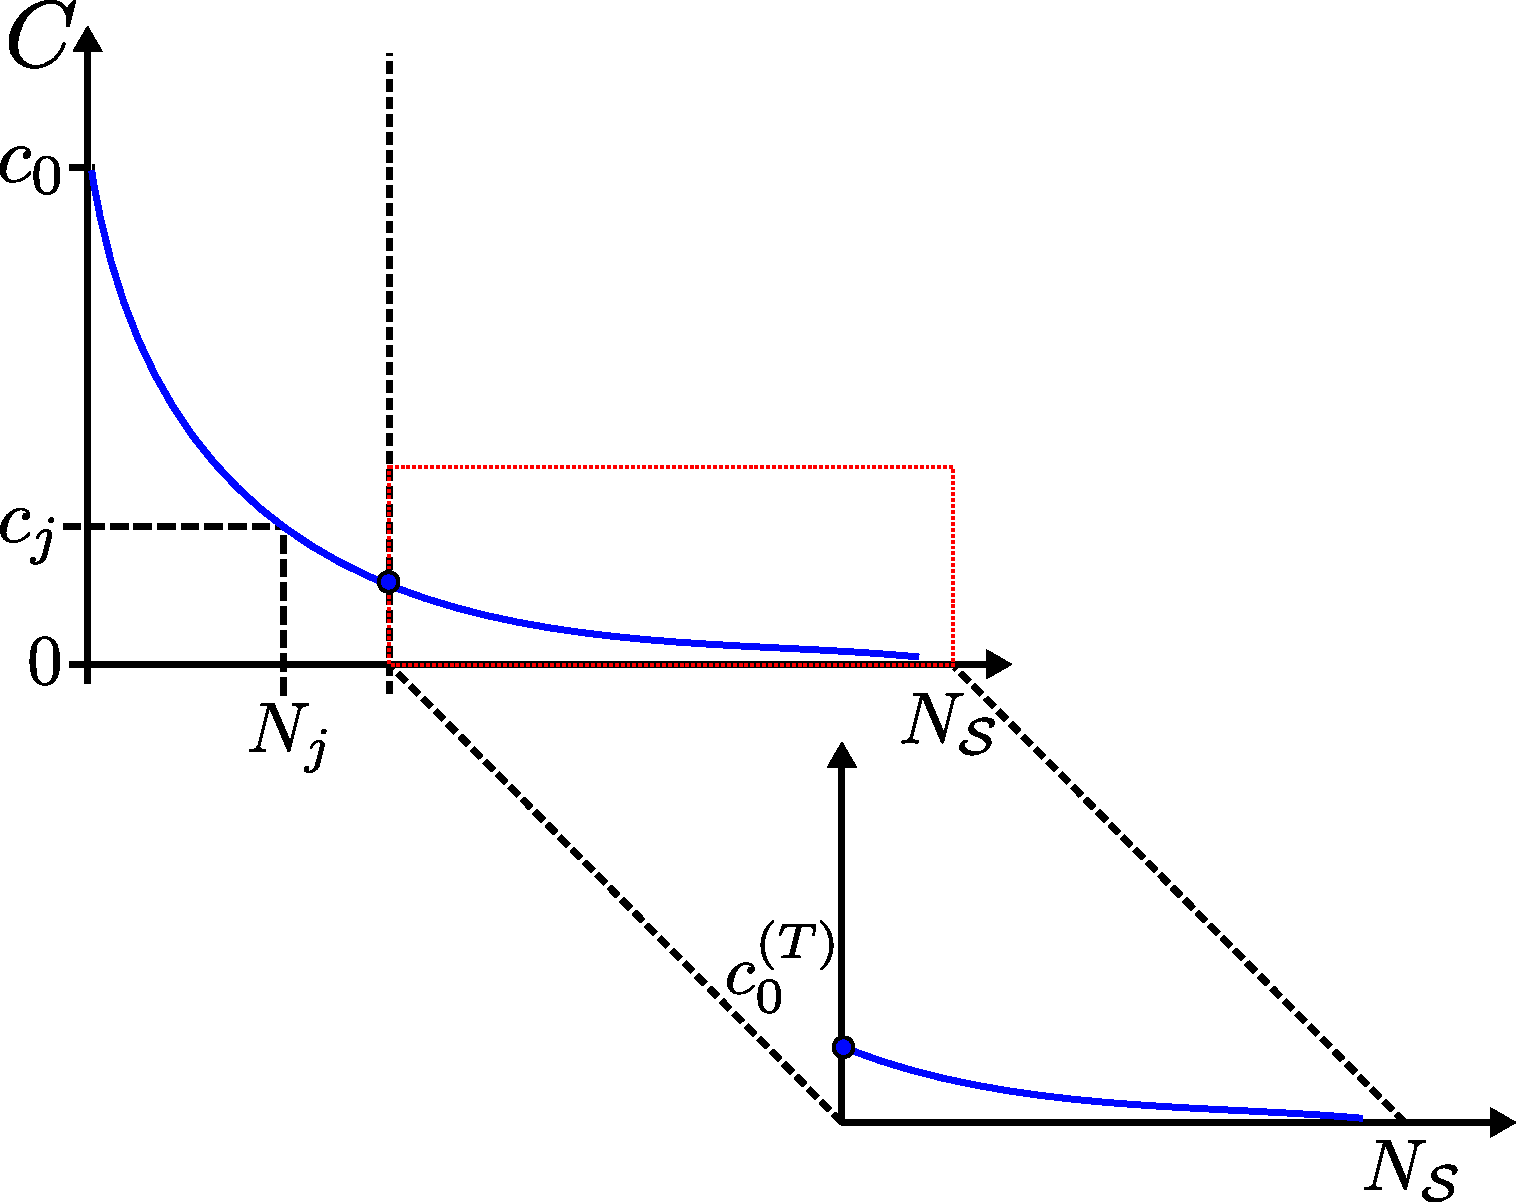
\includegraphics[width=0.9\columnwidth]{fig/effect_transfer_learning.pdf}
%	\caption{The effect of transfer learning.}
%	\label{fig:effect_transfer_learning}
%\end{figure}
%---
TL represents the exchange of knowledge from the skills learned in different \emph{origin} clusters $\mathcal{O}$ to the skills that will be learned in a \emph{target} cluster $\mathcal{T}$, see Fig.~\ref{fig:incremental_transfer_similarity}. In general, the effect that TL has on the skills of another cluster is the reduction of the total remaining knowledge to be learned. Referring to \eqref{eq:incremental_knowledge}, it means that its value when $N_{j,k} = 0$ will be reduced (Fig.~\ref{fig:effect_transfer_learning}). Considering $\mathcal{K} = \{ k_i \}^{N_\mathcal{K}}_{i=1}$ to be the set of all available clusters of knowledge (see Fig.~\ref{fig:cluster_knowledge_transfer}), the TL effect can be modeled as follows
% ---
% \begin{align}
% 	\begin{split}
% 		\bar{\sigma}^{(T)}_{j,k_\mathcal{T}} &= \left\{ e^{-\alpha \left(N_{j,k_\mathcal{T}} - \frac{1}{\alpha \cdot r}  \log\left[ 1- \sum\limits_{k\in \mathcal{K} \setminus k_\mathcal{T}}\beta_k(1 - \bar{\sigma}_{j,k}) \right] \right)}\right\}^r\\
% 		&= \left(e^{-\alpha {N_{j,k_\mathcal{T}}}} \right)^r e^{  \log\left( 1-\sum\limits_{k_\mathcal{O} \in \mathcal{K} \setminus k_\mathcal{T}}\beta_k(1 - \bar{\sigma}_{j,k_{\mathcal{O}}}) \right) }\\
% 		&= \underbrace{\left[1- \sum\limits_{k \in \mathcal{K} \setminus k_\mathcal{T}}\beta_k \left( 1 - \bar{\sigma}_{j,k} \right)\right]}_{\text{Transfer}} \left(e^{-\alpha N_{j,k_\mathcal{T}}} \right)^r ,
% 	\end{split}
% \end{align}


% \begin{align}
% 	\begin{split}
% 		\bar{\sigma}^{(T)}_{j,k_T} &= \left\{ e^{-\alpha \left(N_{j,k_T} - \frac{1}{\alpha \cdot r}  \log\left[ 1- \sum\limits_{k_O\in \mathcal{K} \setminus k_T}\beta_{k_O}\left(1 - \bar{\sigma}_{j,k_O}\right) \right] \right)}\right\}^r\\
% 		&= \left(e^{-\alpha {N_{j,k_T}}} \right)^r e^{ \log\left( 1-\sum\limits_{k_O \in \mathcal{K} \setminus k_T}\beta_{k_O}\left(1 - \bar{\sigma}_{j,k_O}\right) \right) }\\
% 		&= \underbrace{\left[1- \sum\limits_{k_O \in \mathcal{K} \setminus k_T}\beta_{k_O} \left( 1 - \bar{\sigma}_{j,k_O} \right)\right]}_{\text{Transfer}} \left(e^{-\alpha N_{j,k_T}} \right)^r ,
% 	\end{split}
% \end{align}

\begin{align}
	\begin{split}
		\bar{\sigma}^{(T)}_{j,k_T} &= \left\{ e^{-\alpha \left(N_{j,k_T} - \frac{1}{\alpha \cdot r}  \log\left[ 1- \sum\limits_{k_O\in \mathcal{K} \setminus k_T}\beta_{k_O}\left(1 - \bar{\sigma}_{k_O}\right) \right] \right)}\right\}^r\\
		&= \left(e^{-\alpha {N_{j,k_T}}} \right)^r e^{ \log\left( 1-\sum\limits_{k_O \in \mathcal{K} \setminus k_T}\beta_{k_O}\left(1 - \bar{\sigma}_{k_O}\right) \right) }\\
		&= \underbrace{\left[1- \sum\limits_{k_O \in \mathcal{K} \setminus k_T}\beta_{k_O} \left( 1 - \bar{\sigma}_{k_O} \right)\right]}_{\text{Transfer}} \left(e^{-\alpha N_{j,k_T}} \right)^r ,
	\end{split}
\end{align}
% ---
\begin{align}
	\begin{split}
		\bar{\sigma}^{(T)}_{j,k} 
		&= \underbrace{\left[1- \sum\limits_{O = 0}^{k-1}\beta_{O} \left( 1 - \bar{\sigma}_{O} \right)\right]}_{\text{Transfer}} \left(e^{-\alpha N_{j,k}} \right)
	\end{split}
\end{align}

\begin{align}
	\begin{split}
		^{\lvert \lvert}\bar{\sigma}^{(T)}_{j,k} 
		&= \underbrace{\left[1- \sum\limits_{O = 0}^{k-1}\beta_{O} \left( 1 - \bar{\sigma}_{O} \right)\right]}_{\text{Transfer}} \left(e^{-\alpha N_{j,k}/} \right)
	\end{split}
\end{align}
where $0<\beta_{k_O} < 1$ is the transfer coefficient from the different origin clusters $k_{O}$ to the target cluster $k_{T}$\footnote{\textcolor{red}{Once again, since there is no inter-agent exchange of knowledge, $ r = 1 $ in this case.}}. Assuming that the origin clusters have unique knowledge contributions to the target cluster implies that
% ---
\begin{equation}
    \sum\limits_{k_O \in \mathcal{K} \setminus k_T}\beta_{k_O} \leq 1.
\end{equation}
% ---
Furthermore, considering Assumptions~\ref{assumption:cluster_size} and \ref{assumption:cluster_transferability},
% ---
% \begin{equation}
%     \beta_{k_O} = \frac{1}{\text{max}\left(\left\lvert \mathcal{K} \setminus k_{T} \right\rvert,1\right)}
% \end{equation}
\begin{equation}
  \beta_{k_O}=\begin{cases}
    1, & \text{if $\mathcal{K} \setminus k_{T}  = \emptyset$}.\\
    \frac{1}{\left\lvert \mathcal{K} \setminus k_{T} \right\rvert-1^}, & \text{otherwise}.
  \end{cases}
\end{equation}
% ---
The term $ 1 - \bar{\sigma}_{k_O} \approx 1 $ represents the knowledge available from each of the different origin clusters (i.e. after their corresponding skills were learned).
% and $ \bar{\sigma}_{j,k} = \bar{\sigma}_m $. Where $ \bar{\sigma}_m $ represents the knowledge collected from the other clusters; i.e.
% % ---
% \begin{equation}
% 	\bar{\sigma}_m = e^{-\alpha \frac{N_\mathcal{S}}{m N_\mathcal{K}}}.
% \end{equation}
%---
% \begin{figure}[!h]
% 	\centering
% 	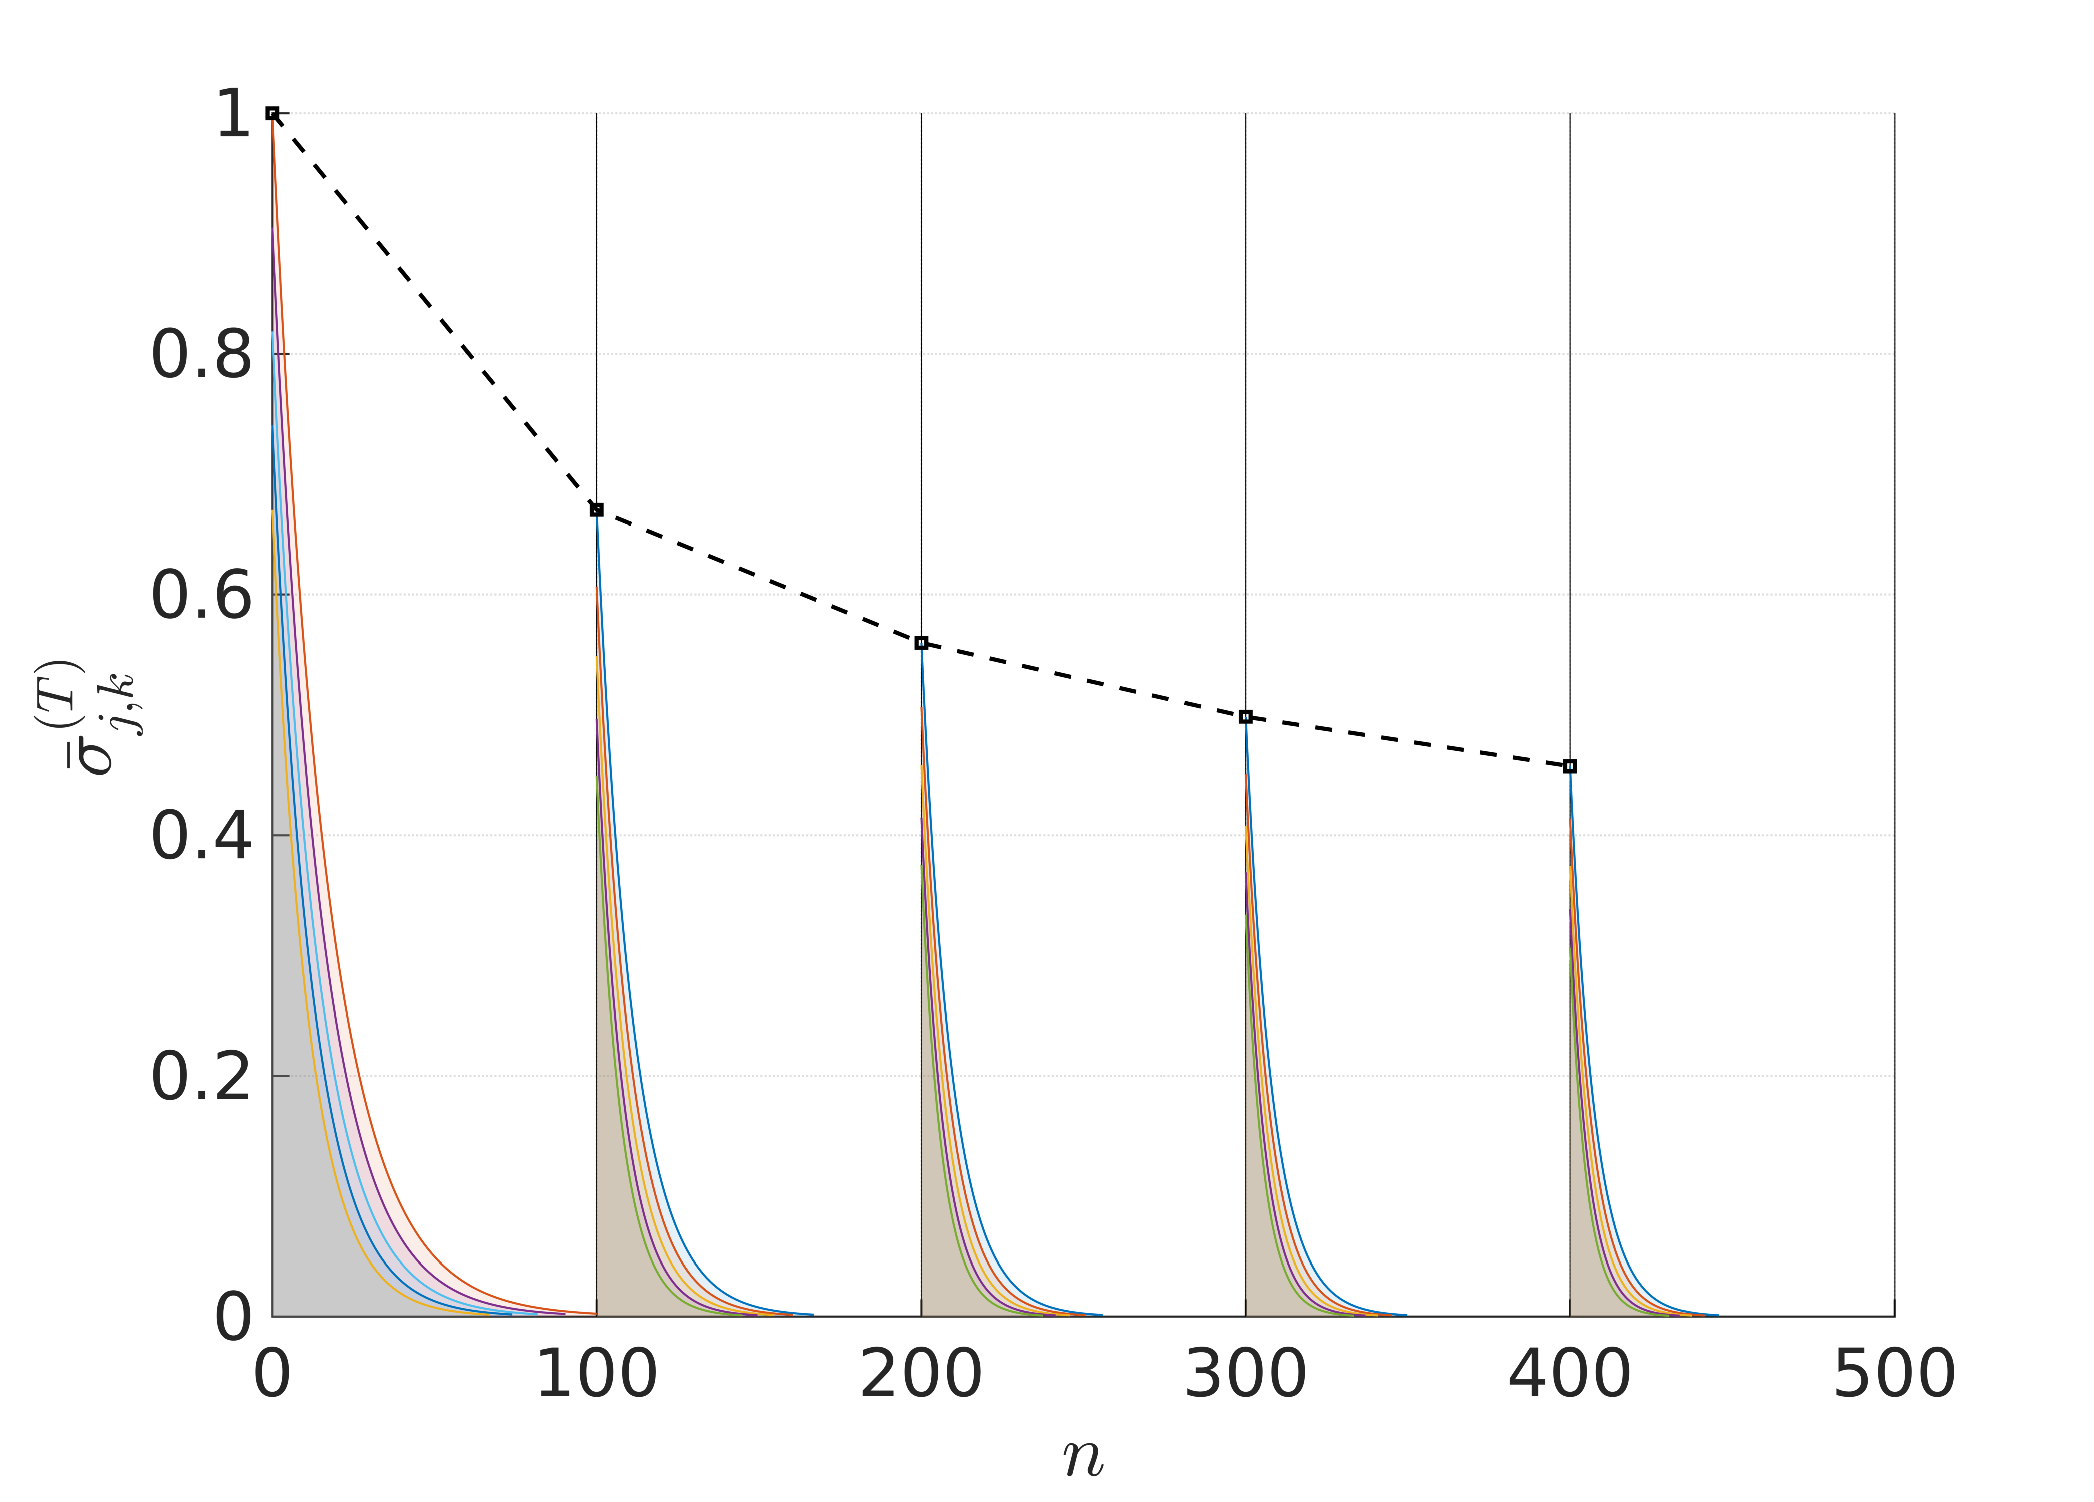
\includegraphics[width=0.99\columnwidth]{tex/fig/single_transfer_knowledge.pdf}
% 	\caption{Knowledge sharing in transfer learning. A single agent leverages previously acquired knowledge from other learned skills in the current and previously learned clusters.}
% 	\label{fig:single_transfer_knowledge}
% \end{figure}
% ---
\begin{figure}[!h]
	\centering
	\includegraphics[width=0.99\columnwidth]{tex/fig/single_transfer_complexity.pdf}
	\caption{Skill complexity is reduced further by the effect of transfer learning as more clusters are visited.}
	\label{fig:single_transfer_complexity}
\end{figure}
% ---
In TL, the skill complexity in the target cluster $k_T$ is then given by
% ---
\begin{equation}
    c^{(T)}_{j,k_T} = c_0 \cdot \bar{\sigma}^{(T)}_{j,k_T},
\end{equation}
% ---
see Fig.~\ref{fig:single_transfer_complexity}. Notice that as the number of seen clusters increases, the starting complexity for the skills in the target cluster is reduced even further. Consequently, similar to incremental learning, the number of trial episodes to learn the skills in the $k_\mathcal{T}$ cluster is
% ---
\begin{align}\label{eq:complexity_transfer_single}
	C_{k}^{(T)} &= \left[1 - \sum_{k_O \in \mathcal{K}\setminus k_T}\beta_{k_O} \left(1-\bar{\sigma}^{(I)}_{k_O}\right)\right]  \cdot  c_0 \frac{1 - e^{-\alpha \frac{N_\mathcal{S}}{N_\mathcal{K}}}}{1 - e^{-\alpha}}
\end{align}
% ---

Consequently, total number of trial episodes required to learn all the skills in the $ N_\mathcal{K} $ clusters is
% ---
\begin{align}\label{eq:complexity_transfer_single}
	C_\mathcal{S}^{(T)} &= \left[1 - \frac{\left(1+N_\mathcal{K}\right)}{2}\beta \left(1-\bar{\sigma}^{(I)}_k\right)\right] N_\mathcal{K} \cdot  c_0 \frac{1 - e^{-\alpha \frac{N_\mathcal{S}}{N_\mathcal{K}}}}{1 - e^{-\alpha}}\\
	&= \left[1 - \frac{\left(1+N_\mathcal{K}\right)}{2}\beta \left(1-\bar{\sigma}^{(I)}_k\right)\right] N_\mathcal{K} \cdot  c_0 \frac{1 - \bar{\sigma}^{(I)}_k}{1 - e^{-\alpha}}	
\end{align}
% ---
Furthermore, if $ m $ robots can be used in parallel to learn the skills in the clusters; then
% ---
\begin{equation}\label{eq:complexity_transfer_parallel}
	{}^{\lvert \lvert}C_\mathcal{S}^{(T)} = \left[1 - \frac{\left(1+N_\mathcal{K}\right)}{2}\beta \left(1-\bar{\sigma}_m\right)\right] m \cdot N_\mathcal{K}  \cdot c_0 \frac{1 - e^{-\alpha \frac{N_\mathcal{S}}{m \cdot N_\mathcal{K}}}}{1 - e^{-\alpha}},
\end{equation}

\begin{tcolorbox}
\begin{align}
	e^{-\gamma \cdot N_j \cdot m}  &= \left[1 - \frac{\left(1+N_\mathcal{K}\right)}{2}\beta \left(1-\bar{\sigma}_m\right)\right]  \cdot m \cdot \frac{1 - e^{-\alpha \frac{N_\mathcal{S}}{m \cdot N_\mathcal{K}}}}{1 - e^{-\alpha}}\\
	\gamma &= -\frac{1}{N_j my}\text{log} \left( \left[1 - \frac{\left(1+N_\mathcal{K}\right)}{2}\beta \left(1-\bar{\sigma}_m\right)\right]  \cdot m \cdot \frac{1 - e^{-\alpha \frac{N_\mathcal{S}}{m \cdot N_\mathcal{K}}}}{1 - e^{-\alpha}}\right)
\end{align}
\end{tcolorbox}
% ---
% ---------------------------------------------------------------------------------------------------
\subsubsection{\textbf{Collective learning (CL)}}
Finally, in collective learning the notion of cluster is not necessarily applicable anymore, thus 
$\mathcal{K} = k_\mathcal{T}$ which corresponds to the existence of only one big cluster.
% ---
\begin{align}
	\begin{split}
		\bar{\sigma}_j^{(C)} &=   \cancelto{1}{ \left[1- \sum_{k_O \in \mathcal{K} \setminus k_T}\beta_{k_O} \left( 1 - \bar{\sigma}_{k_O} \right)\right]} \left(e^{-\alpha {N_{j,k_T}}} \right)^r \\
		&= \left(e^{-\alpha N_{j,k_T}} \right)^r  = \left(e^{-\alpha N_{j}}\right)^r 
	\end{split}
\end{align}

Furthermore, now $m$ robots are learning (potentially) $m$ different skills in parallel while exchanging knowledge.
% ---
\begin{align}\label{eq:collective_knowledge}
\begin{split}
    \bar{\sigma}_i^{(C)} &= \left({e^{-\alpha \cdot N_i}}\right)^{r}\\
    &= \left({e^{-\alpha \cdot N_i}}\right)^{m}.
\end{split}
\end{align}
% ---
The mapping for the $i$-th skill in the universe relative to the $j$-th skill in the $k$-th cluster is
\begin{equation}
    i = (k-1)\frac{N_\mathca{S}}{N_\mathca{K}} + j,k
\end{equation}

%where $\alpha$ was replaced by $ 0<\gamma<<1$, which models a more effective knowledge transfer among the $m$ agents.}
Based on \eqref{eq:collective_knowledge} the scaled down skill complexity in CL is 
% ---
\begin{align}\label{eq:collective_knowledge}
\begin{split}
    ^{||}c_j^{(C)} &= c_o \cdot \left({e^{-\alpha \cdot N_j}}\right)^{m}.
\end{split}
\end{align}
% ---
The total number episodes when using collective learning is given by
% ---
\begin{eqnarray}
	^{||}C_\mathcal{S}^{(C)} = m \cdot C_0 \frac{1 - e^{-\alpha N_\mathcal{S}}}{1 - e^{-\alpha m}}
\end{eqnarray}
% ---
% ===================================================================================================
\subsection{Comparison}
The general skill complexity scaling based on knowledge sharing is given by the following expression
\begin{tcolorbox}
	\begin{align}\label{eq:general_complexity}
		c_{j,k_T} &= c_0\left[1- \sum\limits_{k_O \in \mathcal{K} \setminus k_T}\beta_{k_O} \left( 1 - \bar{\sigma}_{k_O} \right)\right] \left(e^{-\alpha N_{j,k_T}} \right)^r
	\end{align}
\end{tcolorbox}
Expression \ref{eq:general_complexity} can be re written to show the contribution of the different learning schemes as
% ---
\begin{align}
	c_{j,k_T} &= c_0\underbrace{\left[1- \sum\limits_{k_O \in \mathcal{K} \setminus k_T}\beta_{k_O} \left( 1 - \bar{\sigma}^{(I)}_{k_O} \right)\right]}_{TL}\overbrace{ \left(\bar{\sigma}^{(I)}_{j,k_T} \right)^{r-1}}^{CL}\underbrace{ \left(\bar{\sigma}^{(I)}_{j,k_T} \right)}_{IL}
\end{align}
% ---
with
\begin{align}
    \bar{\sigma}^{(I)}_{j,k_T}&= e^{-\alpha N_{j,k_T}},
\end{align}
 where according to \eqref{eq:learning_combinations}, the effects of the different learning schemes are reflected.
 % ---
 \begin{equation}
	 c_j =
	     \begin{cases} 
		       \text{Incremental} & \alpha\neq 0, \beta=0,  r=1 \\
		       \text{Transfer} & \alpha\neq 0, \beta \neq 0, r = 1 \\
		       \text{Collective} & \alpha\neq 0, \beta = 0, r=m 
		   \end{cases}
	   \label{eq:learning_combinations}
\end{equation}
From \eqref{eq:complexity_incremental_parallel} and \eqref{eq:complexity_transfer_parallel} it is clear that they differ only by the factor $ \left[1 - \frac{\left(1+N_\mathcal{K}\right)}{2}\beta \left(1-\bar{\sigma}_m\right)\right] \leq 1$, showing that TL is a scaled down version of IL. Table~\ref{tab:method_comparison} shows the comparison between the total number of trial episodes required by the three learning schemes.

% ---
The total energy and time consumption in the different learning paradigms is
% ---
\begin{align}
	\begin{split}
		E^{(\star)}_{\mathcal{S}} &= e_{0} \cdot {}^{\lvert \lvert}C_\mathcal{S}^{(\star)}\\
		T^{(\star)}_{\mathcal{S}} &= \frac{\Delta t}{m} \cdot {}^{\lvert \lvert}C_\mathcal{S}^{(\star)},
	\end{split}
\end{align}
% -----
with $ \star $ representing the total complexity corresponding the considered learning scheme. Fig.~\ref{fig:energy_time_learning_paradigms} shows the effect in the energy and time demand from the three different learning paradigms as a function of the number of robots learning, considering $c_0 = 100$, $P_0  = \unit[100]{W}$, $ \Delta t = \unit[300]{s}$ and $ N_\mathcal{S} = 10^6 $. In the upper panel of Fig.~\ref{fig:energy_time_learning_paradigms}, it can be seen that the transfer learning paradigm consumes less energy than the incremental one for all cluster size variations. Furthermore, there is a clear upper bound on the energy consumption for learning all skills in $\mathcal{S}$ with the increase of the number of agents $m$. This effect is due to the division of skills among the agents within a cluster; leading to agents accumulating less knowledge before moving to a new cluster. This upper bound is proportional to $c_0$. Additionally, the figure shows the performance of the robots under the collective learning paradigm to be far more efficient than the other IL and TL. On the lower pane  of Fig.~\ref{fig:energy_time_learning_paradigms}, the amount of time required by each agent to learn all skills is shown. Since the amount of time for each trial episode is fixed, we can say that the values are then proportional to the wall-clock time to learn all skills. We can see that, for all paradigms, the more agents we use the faster all skills will be learned, up to a stable point where there is no apparent performance increase by having more agents. Similar to the energy plot, TL is also more efficient than IL, but both are much less efficient than CL. We can further observe that in the collective paradigm there is a quicker saturation of the efficiency, denoting that, even with a relative small number of agents, it should be possible to learn all skills using the same wall-clock time than with a bigger number of agents. This hints at the existence of an optimal trade-off between the number of agents and the time required to learn a given number of skills.
% ---
% \begin{figure*}[!htb]
% 	\centering
% 	\hspace*{\fill}
% 	\subfloat[]{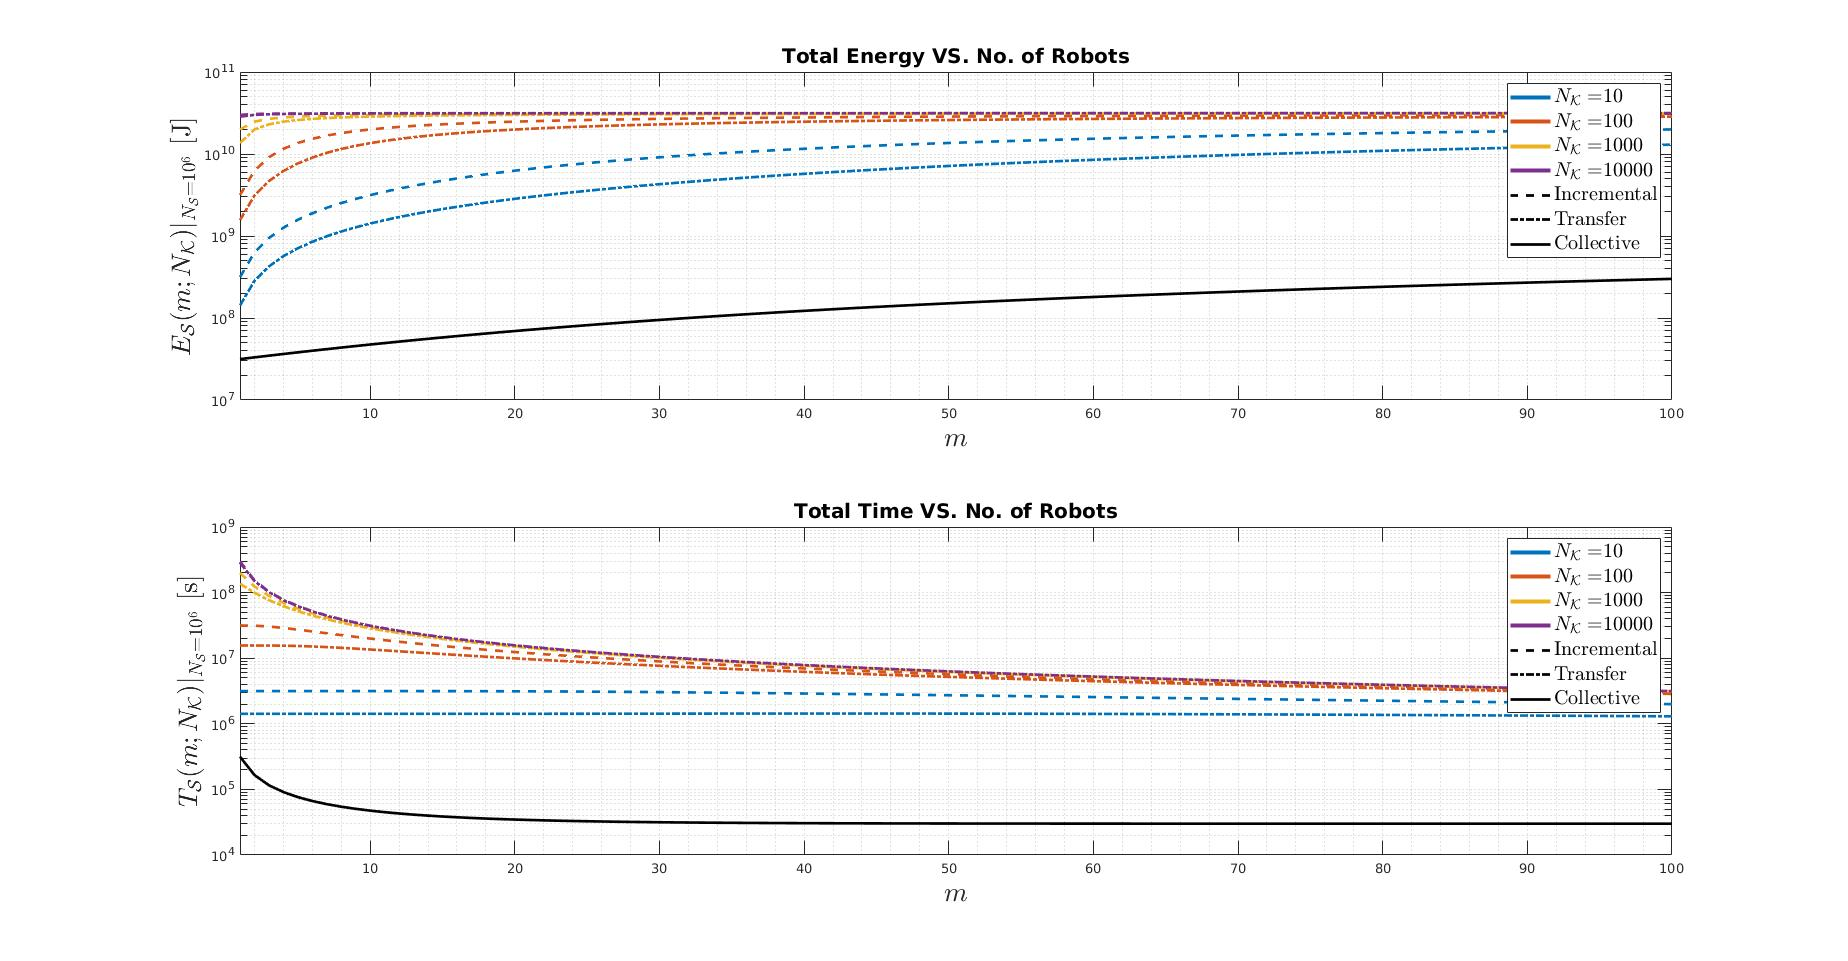
\includegraphics[width= 0.99\textwidth]{fig/energy_time_learning_paradigms.jpg}}  
% 	\hspace*{\fill}
% 	\caption[] {\label{fig:energy_time_learning_paradigms} The total energy and time demands for the different learning paradigms, considering $ N_\mathcal{S} = 10^6 $.}
% \end{figure*}
% ---
%---
\begin{figure*}[!htb]
	\centering
	\hspace*{\fill}
	\subfloat[]{\includegraphics[width= 0.30\textwidth]{fig/complexity_incremental.pdf} \label{fig:complexity_incremental}}  
	\hfill
	\subfloat[]{\includegraphics[width= 0.30\textwidth]{fig/single_transfer_complexity.pdf} \label{fig:single_transfer_complexity}}  
	\hfill	
	\subfloat[]{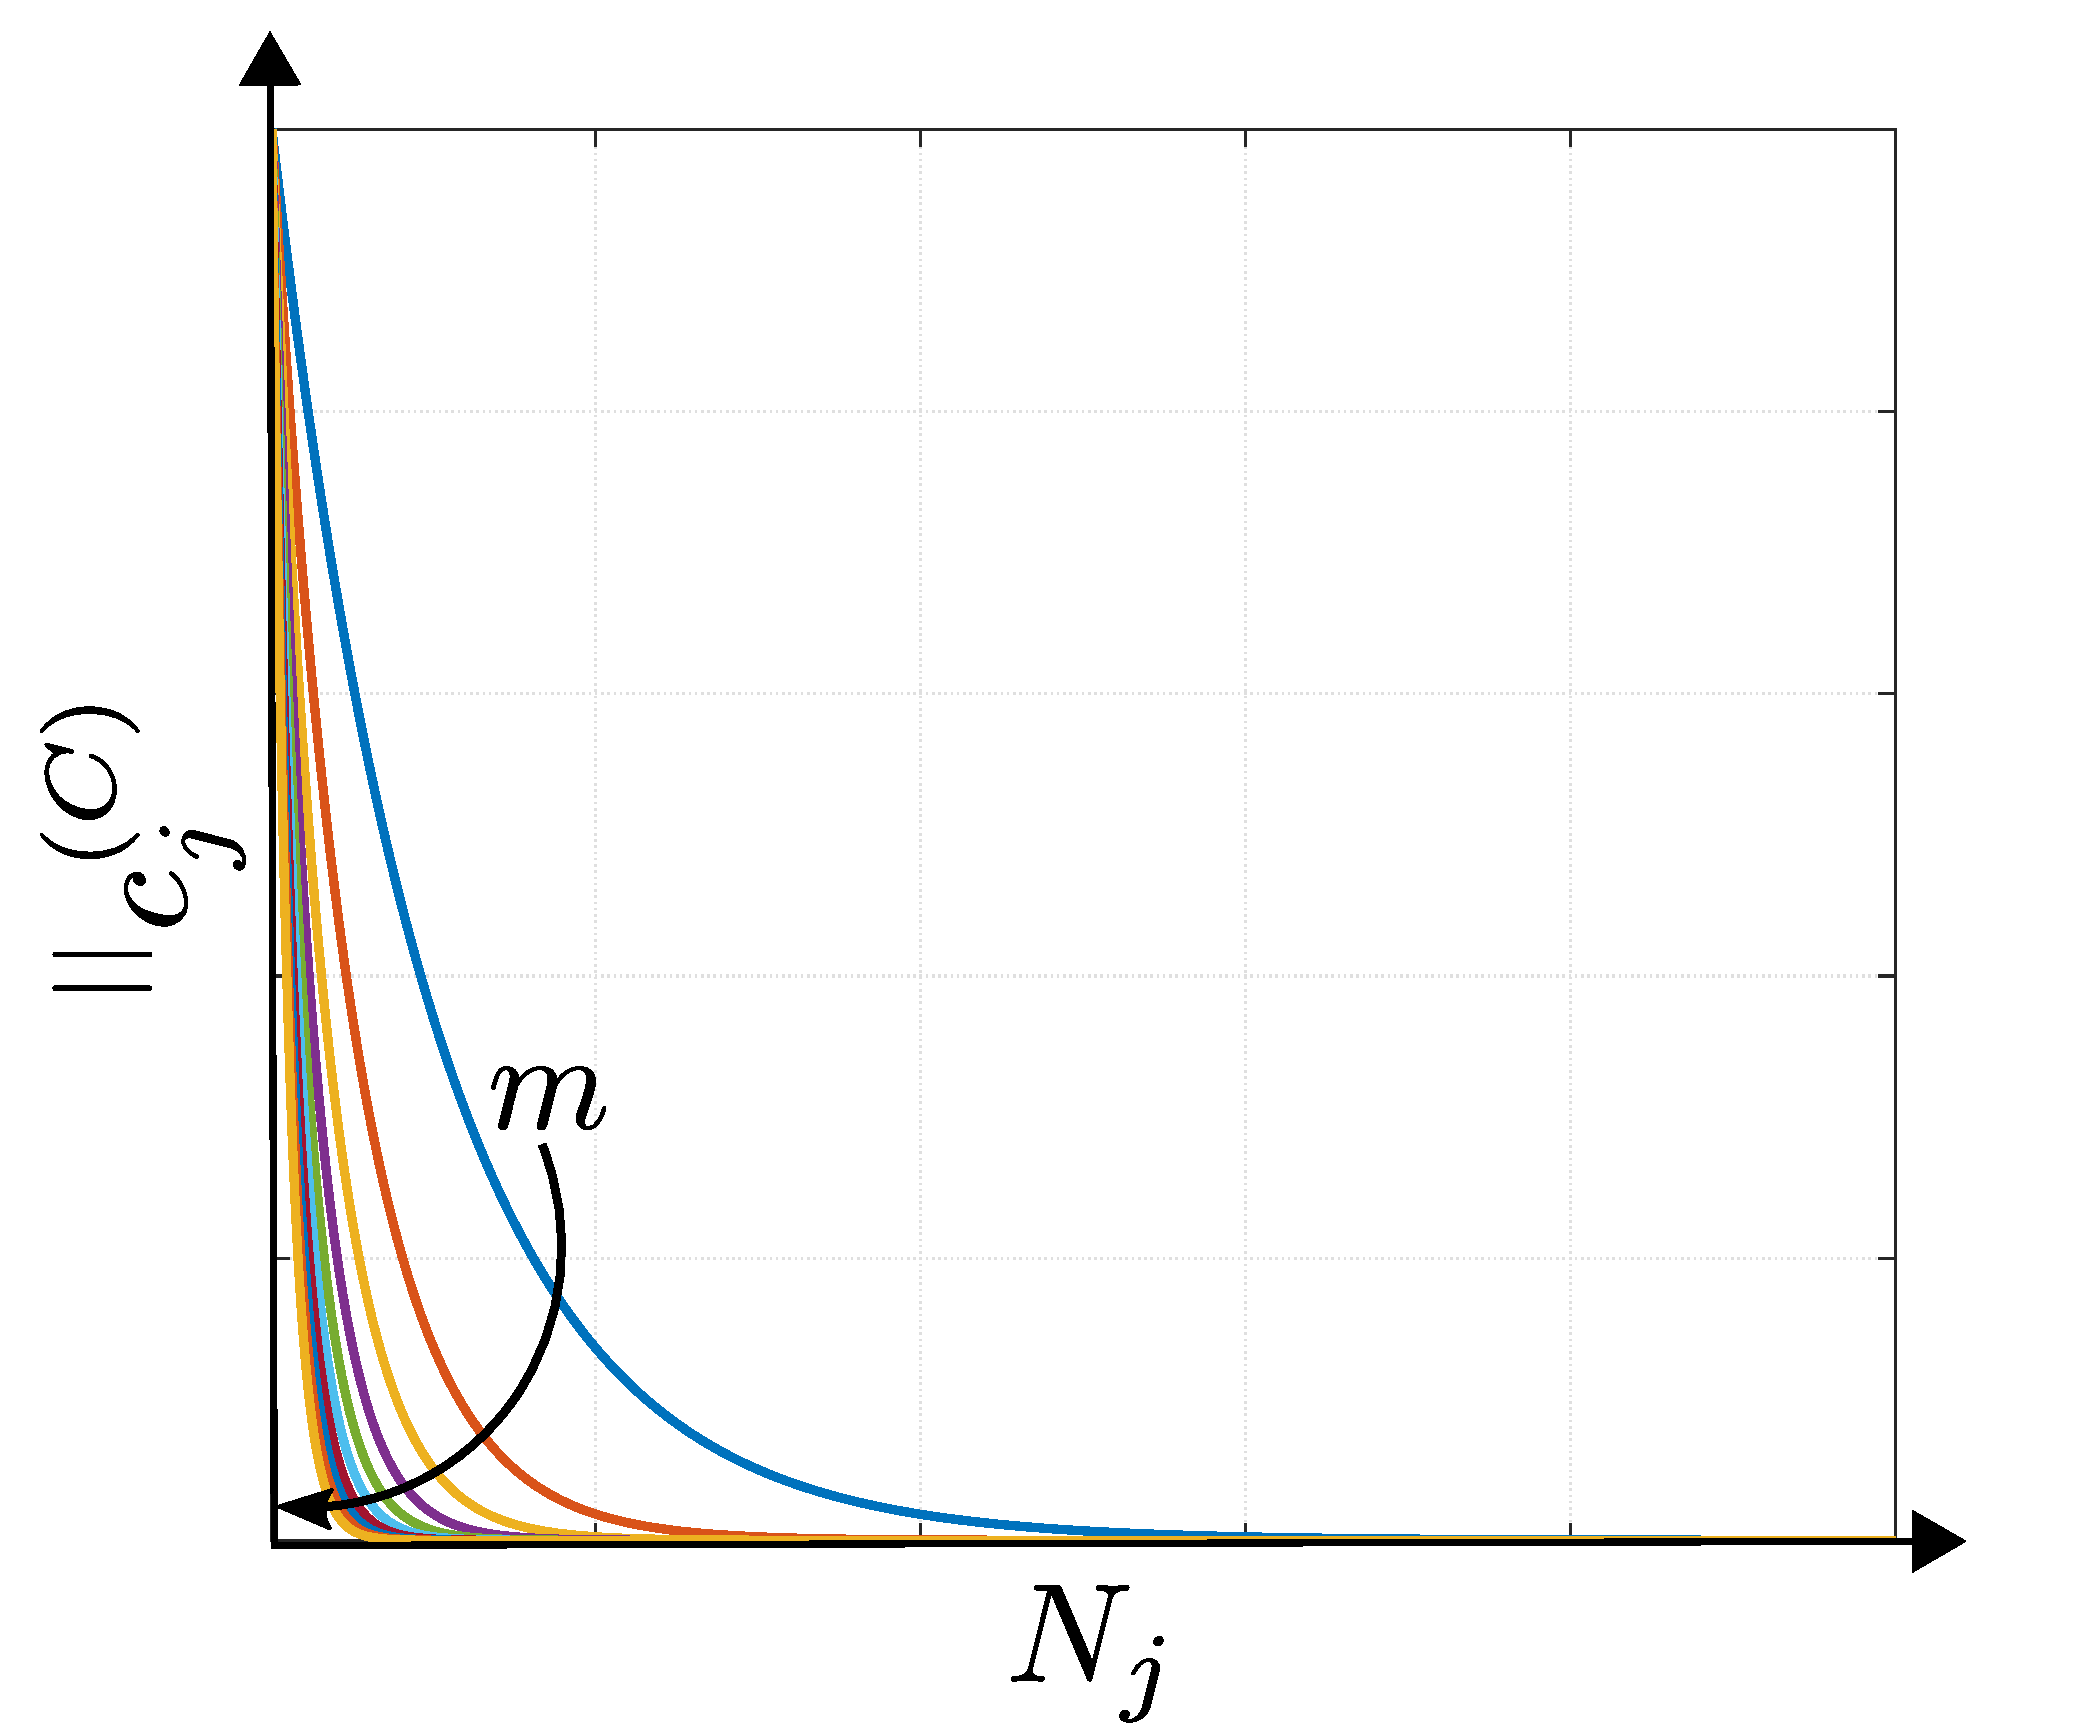
\includegraphics[width= 0.30\textwidth]{tex/fig/collective_complexity.pdf} \label{fig:collective_complexity}}
	\hspace*{\fill}
	\caption[] {\label{fig:energy_time_learning_paradigms} Transfer learning. \subref{fig:effect_transfer_learning} The total \subref{fig:parallel_total_energy} energy and \subref{fig:parallel_total_time} time demands for the different learning paradigms, considering $ N_\mathcal{S} = 10^6 $.}
\end{figure*}
% ---
\begin{figure*}[!htb]
	\centering
	\hspace*{\fill}
	\subfloat[]{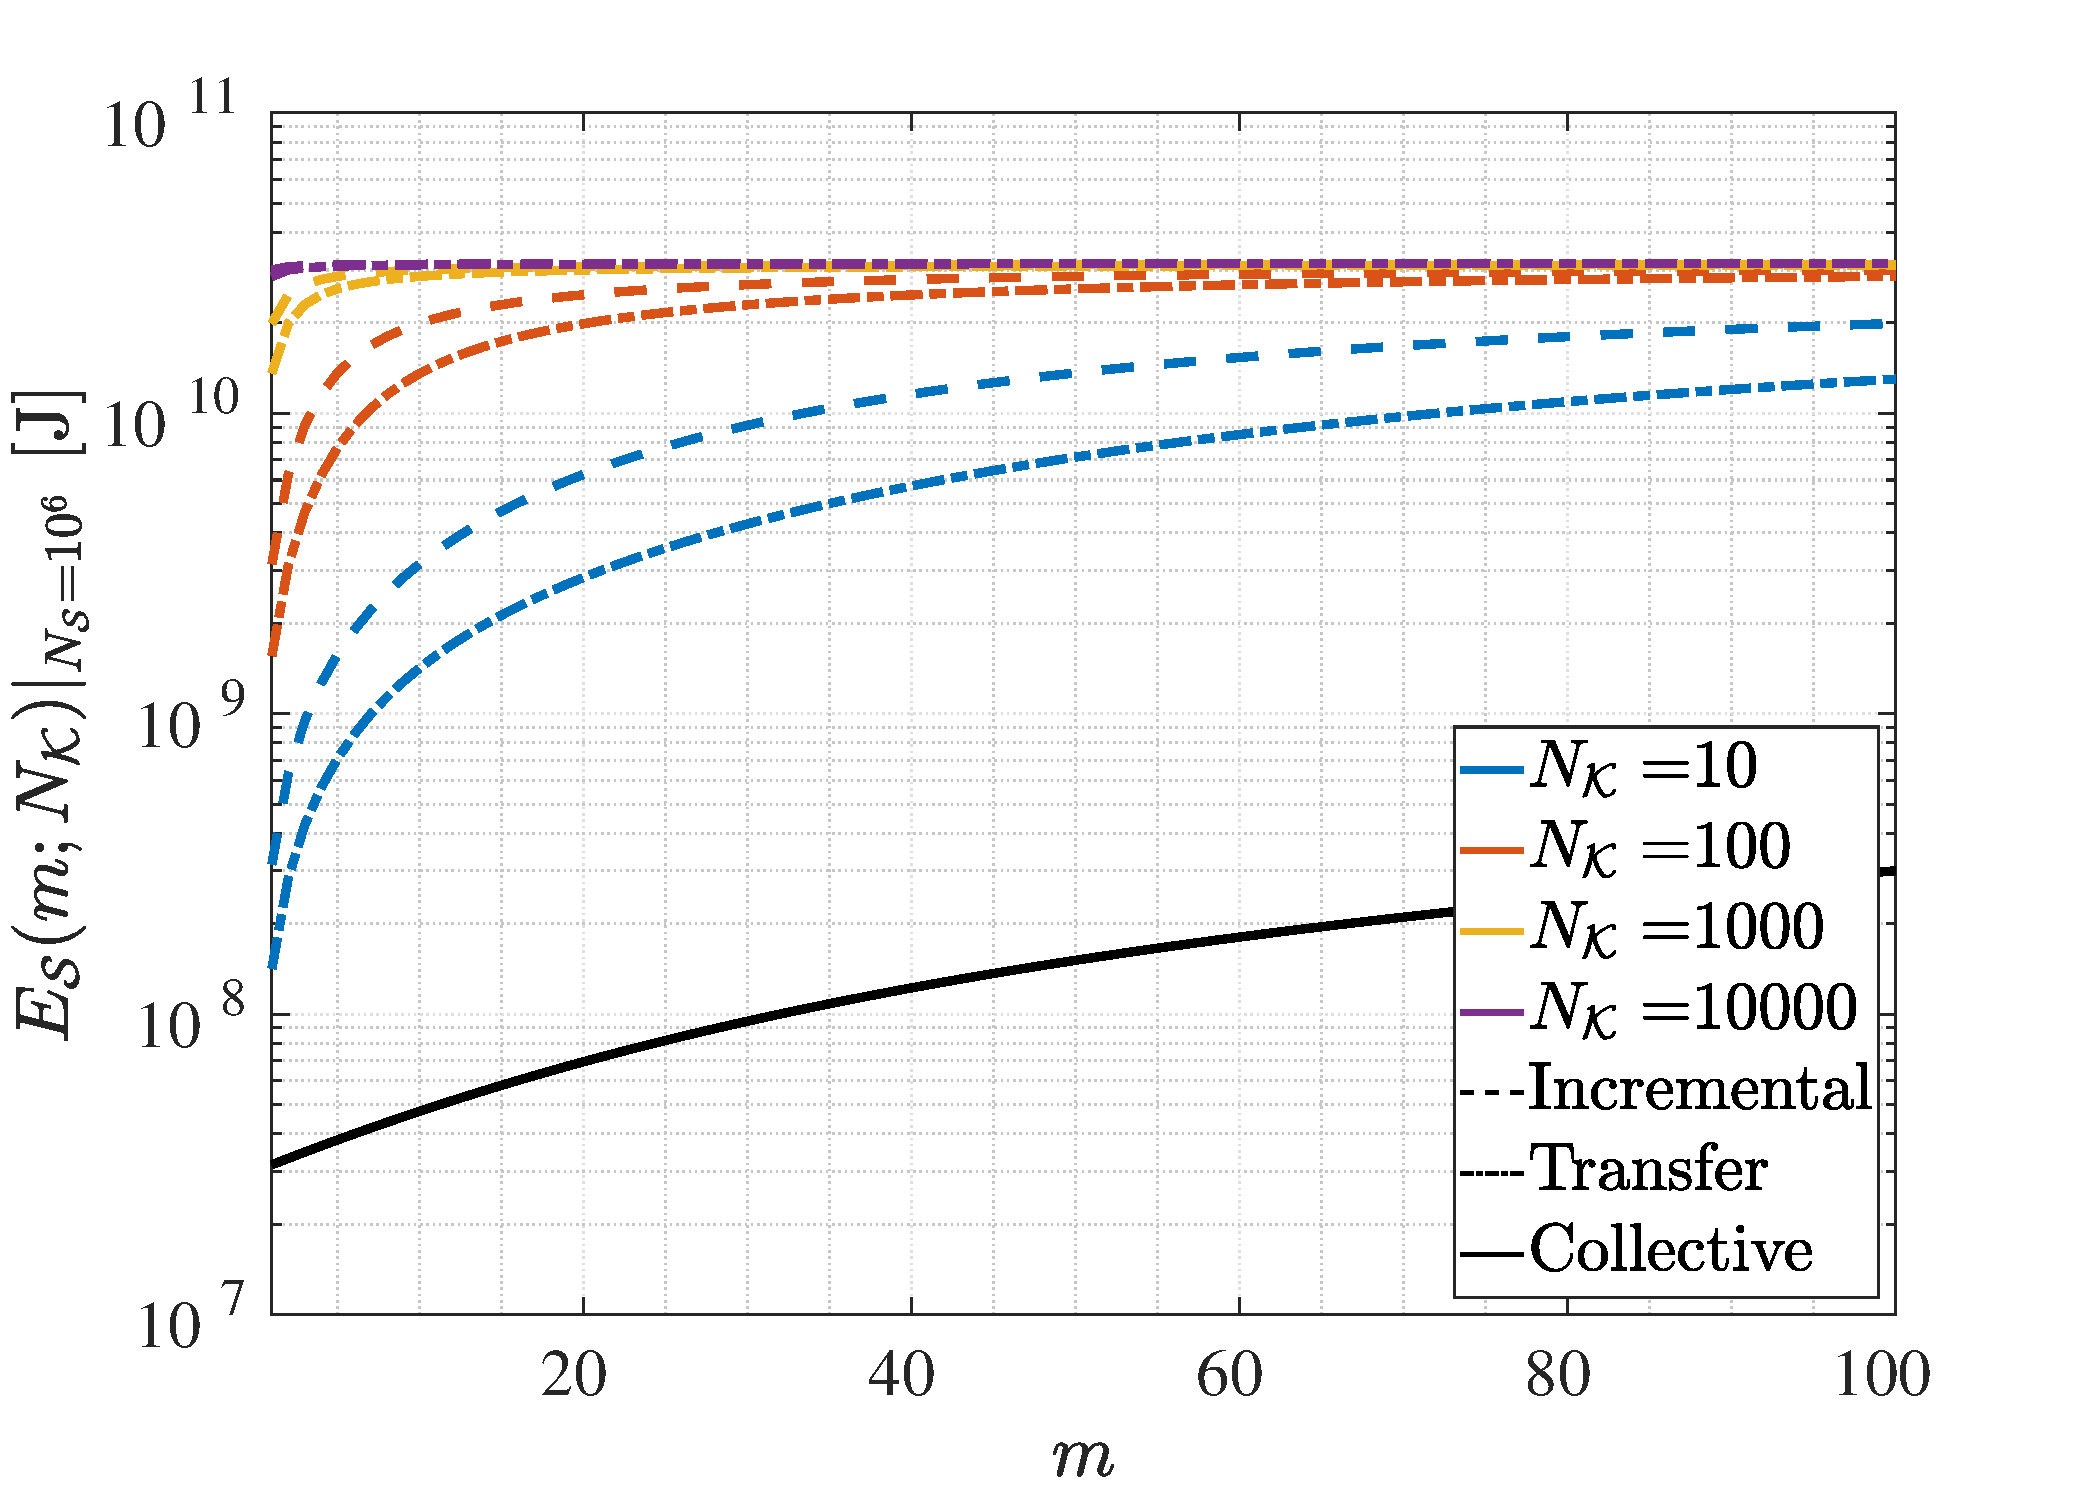
\includegraphics[width= 0.90\columnwidth]{fig/parallel_total_energy.pdf} \label{fig:parallel_total_energy}}  
	\hfill
	\subfloat[]{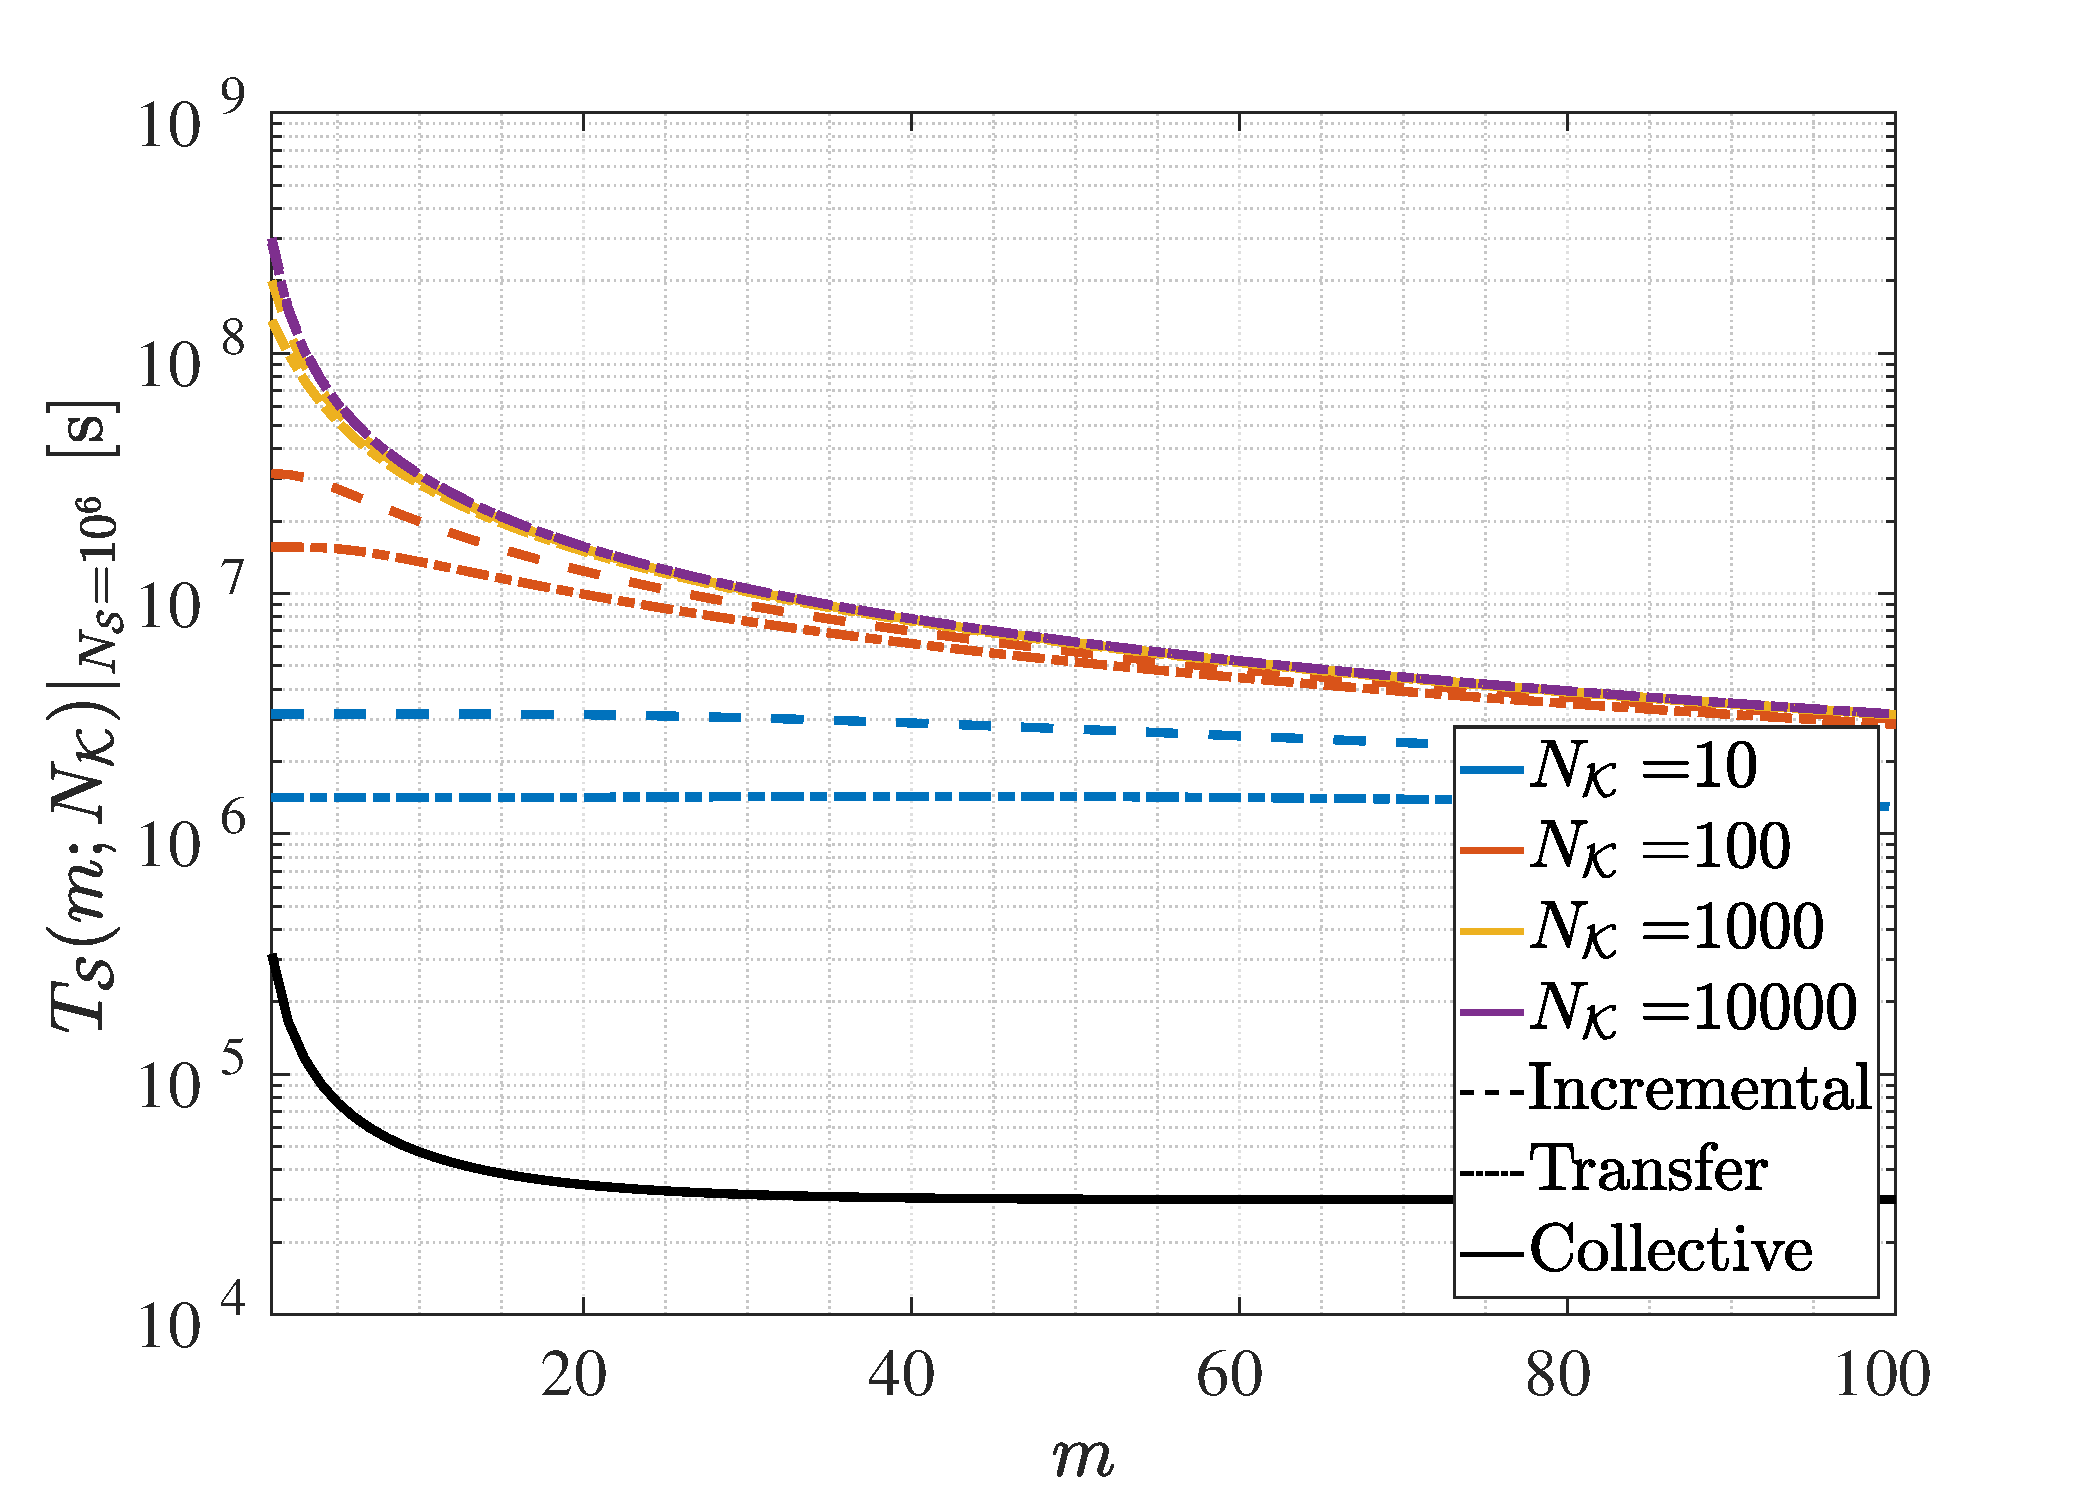
\includegraphics[width= 0.90\columnwidth]{fig/parallel_total_time.pdf} \label{fig:parallel_total_time}}
	\hspace*{\fill}
	\caption[] {\label{fig:energy_time_learning_paradigms} Transfer learning. \subref{fig:effect_transfer_learning} The total \subref{fig:parallel_total_energy} energy and \subref{fig:parallel_total_time} time demands for the different learning paradigms, considering $ N_\mathcal{S} = 10^6 $.}
\end{figure*}